
%  Created by Colin Williams on 2012-01-06.
%  Copyright (c) 2012 __MyCompanyName__. All rights reserved.
%
\documentclass[]{article}

% Use utf-8 encoding for foreign characters
\usepackage[utf8]{inputenc}

% the page geometry.
\usepackage[a4paper,top=2cm, bottom=2cm, left=1cm, right=1cm]{geometry}

% Uncomment some of the following if you use the features
%
% Running Headers and footers
%\usepackage{fancyhdr}

% Multipart figures
%\usepackage{subfigure}

% More symbols
%\usepackage{amsmath}
%\usepackage{amssymb}
%\usepackage{latexsym}

% Surround parts of graphics with box
\usepackage{boxedminipage}

% Package for including code in the document
\usepackage{listings}

% If you want to generate a toc for each chapter (use with book)
\usepackage{minitoc}

% This is now the recommended way for checking for PDFLaTeX:
\usepackage{ifpdf}
\usepackage{comment}

%\newif\ifpdf
%\ifx\pdfoutput\undefined
%\pdffalse % we are not running PDFLaTeX
%\else
%\pdfoutput=1 % we are running PDFLaTeX
%\pdftrue
%\fi


\usepackage{array}
\usepackage{url}
\usepackage{listings}
\usepackage{color}
\usepackage{amsmath}
\usepackage{mathtools}

% clickable links in the contents section
\usepackage{hyperref}
\hypersetup{
    colorlinks,
    citecolor=black,
    filecolor=black,
    linkcolor=black,
    urlcolor=black
}


\definecolor{dkgreen}{rgb}{0,0.6,0}
\definecolor{gray}{rgb}{0.5,0.5,0.5}
\definecolor{mauve}{rgb}{0.58,0,0.82}


\newcommand*\vtick{\textsc{\char13}}

\lstset{
  language=Java,
  tabsize=4,
  showstringspaces=false,
  basicstyle=\tt,
  numberstyle=\tiny\color{gray},      % line number style
  keywordstyle=\color{blue},          % keyword style
  commentstyle=\color{dkgreen},       % comment style
  stringstyle=\color{mauve},          % string literal style
}

\ifpdf
\usepackage[pdftex]{graphicx}
\else
\usepackage{graphicx}
\fi

% this gives us \FloatBarrier to prevent images to float all to the end
\usepackage{placeins}

\title{Negotiation User Guide}
\author{T. Baarslag, W. Pasman, K. Hindriks, D. Tykhonov, W. Visser, M. Hendrikx, D. Feirstein}

\date{\today}

% Alter some LaTeX defaults for better treatment of figures:
    % See p.105 of "TeX Unbound" for suggested values.
    % See pp. 199-200 of Lamport's "LaTeX" book for details.
    %   General parameters, for ALL pages:
    \renewcommand{\topfraction}{0.9}	% max fraction of floats at top
    \renewcommand{\bottomfraction}{0.8}	% max fraction of floats at bottom
    %   Parameters for TEXT pages (not float pages):
    \setcounter{topnumber}{2}
    \setcounter{bottomnumber}{2}
    \setcounter{totalnumber}{4}     % 2 may work better
    \setcounter{dbltopnumber}{2}    % for 2-column pages
    \renewcommand{\dbltopfraction}{0.9}	% fit big float above 2-col. text
    \renewcommand{\textfraction}{0.07}	% allow minimal text w. figs
    %   Parameters for FLOAT pages (not text pages):
    \renewcommand{\floatpagefraction}{0.7}	% require fuller float pages
	% N.B.: floatpagefraction MUST be less than topfraction !!
    \renewcommand{\dblfloatpagefraction}{0.7}	% require fuller float pages

	% remember to use [htp] or [htpb] for placement
	
\begin{document}

\ifpdf
\DeclareGraphicsExtensions{.pdf, .jpg, .tif}
\else
\DeclareGraphicsExtensions{.eps, .jpg}
\fi

\maketitle

\newcommand\Genius{{\sc Genius\ }}

\abstract{\noindent \Genius \cite{Genius}~is a negotiation environment that implements an open architecture for heterogeneous negotiating agents. \Genius~can be used to implement, or simulate, real life negotiations. This document describes how you can install the environment, work with the provided scenarios and negotiation agents, and write, compile, and run an agent yourself.}

\pagebreak
\tableofcontents

\pagebreak


%=========================================================================================
\section{Theory Crash Course}
This section provides a crash course on some essential theory needed to understand the negotiation system. Furthermore, it provides an overview of the features of a negotiation implemented in \Genius.

\subsection{Negotiation Objects}
Parties participating in a negotiation interact in a domain. The domain specifies the possible bids. The parties all have their own preferences, which is reflected in their profile.  Figure~\ref{Fig:domain} shows a picture of a domain that describes the issues in the negotiation.

\begin{figure}[htb]
	\centering
	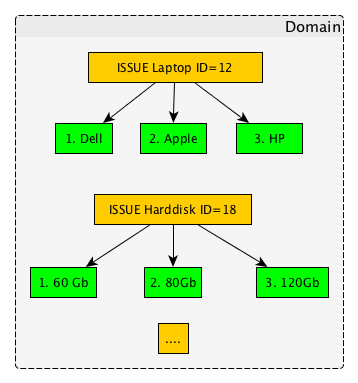
\includegraphics[width=0.4\textwidth]{media/domain.png}
	\caption{An example domain for laptop negotiation. Issues are orange, values are green}\label{Fig:domain}
\end{figure}

The \textit{Domain} describes which issues are the subject of the negotiation and which values an issue can attain. A domain contains $n$ issues: $D=(I_1,\ldots,I_n)$. Each issue $i$ consists of $k$ values: $I_i=(v^i_1,\ldots,v^i_k)$.  Combining these concepts, an agent can formulate a \textit{Bid}: a mapping from each issue to a chosen value (denoted by $c$), $b=(v^i_{c},\ldots,v^n_{c})$. 

To give an example, in the laptop domain the issues are ``laptop'', ``harddisk'' and ``monitor''. In this domain the issues can only attain discrete values, e.g. the ``harddisk'' issue can only have the values ``60 Gb'', ``80 Gb'' and ``120 Gb''. These issues are all instance of \textit{IssueDiscrete}. A valid bid in the laptop domain is a Dell laptop with 80 Gb and a 17' inch monitor.

The \textit{Utility Space} specifies the preferences of the bids for an agent using an evaluator. It is basically just a function that maps bids into a real number in the range [0,1] where 0 is the minimum utility and 1 is the maximum utility of a bid.

A common form of the Utility space is the \textit{Additive Utility Space}. Such a space is additive because each of the issues in the domain have their own utility of their own. For instance, we like Apple with 0.7 and Dell with 0.4, completely independent of how much memory the computer has. Figure~\ref{Fig:utilspace} shows a picture of a utility space for the example domain that we gave above.

\begin{figure}[htb]
	\centering
	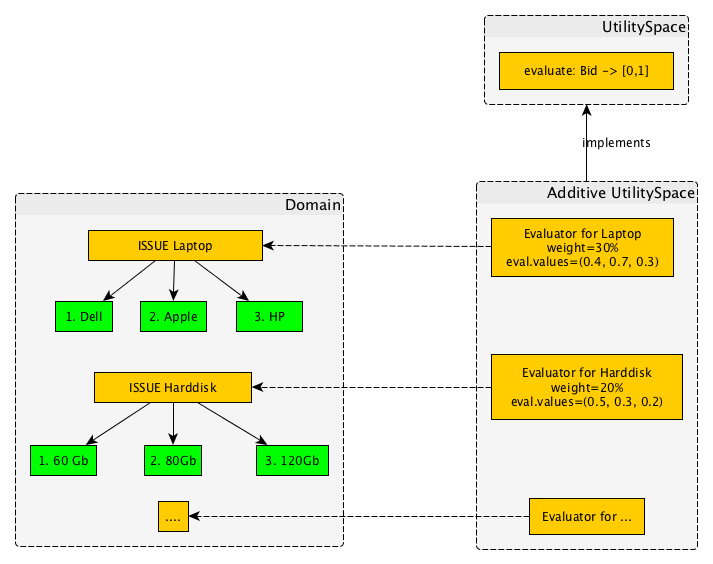
\includegraphics[width=0.6\textwidth]{media/utilspace.png}
	\caption{An example additive utility space for the laptop domain.}\label{Fig:utilspace}
\end{figure}
 
In an additive space the evaluator also specifies the importance of the issue relative to the other issues in the form of a weight. The weights of all issues sum up to 1.0 to simplify calculating the utility of a bid. The utility is the weighted sum of the scaled evaluation values.

\begin{equation}
	U(v^i_{c},\ldots,v^n_{c}) = \sum_{i=1}^{n} w_i \dfrac{\text{eval}(v^i_{c})}{\text{max}(\text{eval}(I_i))}
	\label{eqn:Utility}
\end{equation}


\subsection{Optimality of a Bid}
In general, given the set of all bids, there are a small subset of bids which are more preferred as outcomes by both agents. Identifying these special bids may lead to a better agreement for both parties.

For a single agent, the optimal bid is of maximum utility for the agent. Often this bid has a low utility for the other party, and therefore the chance of agreement is low. A more general notion of optimality of a negotiation involves the utility of both agents.

\begin{figure}[htb]
	\centering
	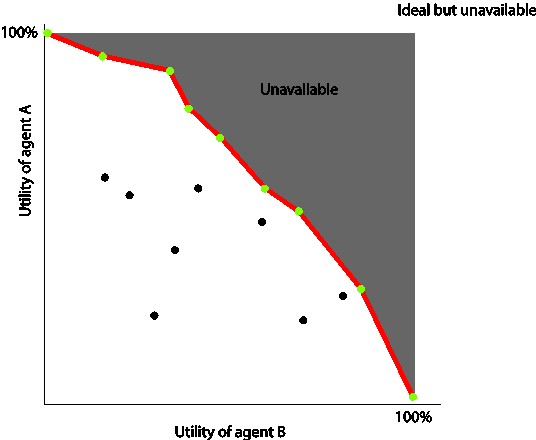
\includegraphics[width=0.37\textwidth]{media/image5.png}
\caption{A point indicates the utility for both agents of a bid. The red line is the Pareto optimal frontier.}\label{Fig:utility plot}
\end{figure}

There are multiple ways to define a more global ``optimum''. One approach to optimality is that a bid is not optimal for both parties if there is another bid that has the higher utility for one party, and at least equal utility for the other party. Thus, only bids in Figure~\ref{Fig:utility plot} for which there is no other bid at the top right is optimal. This type of optimality is called Pareto optimality and forms an important concept in automated negotiation. The collection of Pareto optimal bids is called the Pareto optimal frontier.

A major challenge in a negotiation is that agents can hide their preferences. This entails that an agent does not know which bid the opponent prefers given a set of bids. This problem can be partly resolved by building an \textit{opponent model} of the opponent's preferences by analyzing the negotiation trace. Each turn the agent can now offer the best bid for the opponent given a set of similar preferred bids. \Genius  provides a number of components that can estimate an opponent model.

\subsection{Negotiation Protocol}
The negotiation protocol determines the overall order of actions during a negotiation. Agents are obliged to stick to this protocol, as deviations from the protocol are caught and penalized. \Genius supports multiple protocols. These are discussed in detail in section \ref{sec:protocols}.

 
\subsection{Reservation Value}
A reservation value is a real-valued constant that sets a threshold below which a rational agent should not accept any offers. Intuitively, a reservation value is the utility associated with the Best Alternative to a Negotiated Agreement (BATNA).

A reservation value is the minimum acceptable utility, offers with a utility would normally not be accepted by an agent. Reservation values typically differ for each negotiation agent. In case no reservation value is set in a profile, it is assumed to be 0. Notice that if a negotiation ends with no agreement, agents normally get a utility of 0, regardless of the reservation value.

\subsection{Time Pressure}
A negotiation lasts a predefined time in seconds, or alternatively rounds. In \Genius~the time line is \emph{normalized}, i.e.: time $t \in [0, 1]$, where $t = 0$ represents the start of the negotiation and $t = 1$ represents the deadline. Notice that manipulation of the remaining time can be a factor influencing the outcome.

There is an important difference between a time-based and rounds-based protocol. In a time-based protocol the computational cost of an agent should be taken into account as it directly influences the amount of bids which can be made. In contrast, for a rounds-based negotiation the time can be thought of as paused within a round; therefore computational cost does not play a role.

Apart from a deadline, a scenario may also feature \emph{discount factors}. Discount factors decrease the utility of the bids under negotiation as time passes. While time is shared between both agents, the discount generally differs per agent. 
The default implementation of discount factors is as follows: let $d$ in $[0, 1]$ be the discount factor that is specified in the preference profile of an agent; let $t$ in $[0, 1]$ be the current normalized time, as defined by the timeline; we compute the discounted utility $U_D^t$ of an outcome $\omega$ from the undiscounted utility function $U$ as follows:
\begin{eqnarray}
U_D^t(\omega) = U(\omega) \cdot d^t
\end{eqnarray}
If $d = 1$, the utility is not affected by time, and such a scenario is considered to be undiscounted, while if $d$ is very small there is high pressure on the agents to reach an agreement. Note that discount factors are part of the preference profiles and therefore different agents may have a different discount factor.

If a discount factor is present, reservation values will be discounted in exactly the same way as the utility of any other outcome. It is worth noting that, by having a discounted reservation value, it may be rational for an agent to end the negotiation early and thereby default to the reservation value.
 
%=========================================================================================
\section{Protocols}\label{sec:protocols}
This section describes the various negotiation protocols. The protocol determines the overall order of actions during a negotiation.
This section focuses on the MultiParty protocols as these have been properly developed. There is also a protocol class for the bilateral negotiation, but this is basically a hard coded Stacked Alternating Offers Protocol and not further developed. 

  The (Multilateral)  protocol describes if the negotiation is finished, what the agreement is, which actions can be done in the next round.   Briefly, to run a session the system checks with the protocol if the negotiation is already finished,  and if not which calls need to be made to the parties (both chooseAction and receiveMessage).  We recommend checking the javadoc of MultilateralProtocol for up-to-date detail information and how the protocol is used by the system to run sessions.
  
 The Multilateral protocol uses the notion of rounds and turns to describe the negotiation layout. A round is a part of the negotiation where all participants get a turn to respond to the current state of the negotiation. A turn refers to the opportunity of one party to make a response to the current state of the negotiation. 
  
If an agent violates the protocol -- for instance by sending an action that is not one of the allowed ones, or by crashing, the negotiation ends and the outcome usually is 'no agreement' for all parties.  In bilateral negotiation we have a special case then: the agent's utility is set to its reservation value, whereas the opponent is awarded the utility of the last offer.

All protocols are found in the package \verb|negotiator.protocol| and have the names matching the subsections below.


\subsection{Stacked Alternating Offers Protocol}
According to this protocol \cite{MultilateralOffersProtocols} , all of the participants around the table get a turn per round. Turns are taken clock-wise around the table. One of the negotiating parties starts the negotiation with an offer that is observed by all others immediately. Whenever an offer is made, the next party in line gets a call to receiveMessage containing the bid, followed by a call to chooseAction from which it can return the following actions:
\begin{itemize}
\item Accept the offer (not available the very first turn). 
\item send an Offer to make a counter offer (thus rejecting and overriding the previous offer, if there was any) 
\item send an EndNegotiation and ending the negotiation without any agreement.
\end{itemize}

This protocol is the default protocol for Parties (as returned by getProtocol()).


\subsection{Alternating Multiple Offers Protocol}
According to this protocol \cite{MultilateralOffersProtocols} , all agents have a bid from all agents available to them, before they vote on these bids. This implemented in the following way: The protocol has a bidding phase followed by voting phases. In the bidding phase all participants put their offer on the table. These offers appear to all agents through receiveMessage() in a specific order. In the voting phases all participants vote on all of the bids on the negotiation table, in the same order as received. For each offer, the agent chooseAction() is called. If one of the bids on the negotiation table is accepted by all of the parties, then the negotiation ends with this bid. 

In each even round (we start in round 0), each party gets only one turn for an OfferForVoting. 

In each odd round there are N voting turns for each party (N being the number of offers), one for each offer in order of reception. these are the available options:
\begin{itemize}
\item Accept the offer
\item Reject the offer
\end{itemize}


\subsection{Alternating Majority Consensus Protocol}

This protocol is essentially equal to the Alternating Multiple Offers Protocol, but now an offer the protocol keeps track of the acceptable offer that got most accepts.
Initially, this may be the first offer that got one accept. After a number of rounds, some offers receive multiple accepts and these then become the new acceptable offer.

If an offer is accepted by all parties, the negotiation ends. Otherwise, the negotiation continues (unless the deadline is reached). If the deadline is reached, the acceptable offer becomes the agreement.
 
 
\subsection{Simple Mediator Based Protocol}
In this protocol, the parties do not hear the other parties directly. Instead, they only hear the mediator and the mediator hears the bids of all the parties. The mediator determines which bid will be voted on, collects the votes and determines the outcome. The mediator is just another NegotiationParty, but it extends Mediator.

The protocol requires that exactly one party is a Mediator. The \Genius GUI enforces this presence of a Mediator. When you run a negotiation from the command line you have to ensure the presence of a single Mediator.

This protocol uses the following turns in every round:
\begin{enumerate}
\item Mediator proposes an OfferForVoting
\item The other parties (not the mediator) place a VoteForOfferAcceptance on the OfferForVoting
\item The mediator makes a InformVotingResult that informs all parties about the outcome of this round.
\end{enumerate}

With this protocol, the last InformVotingResult with an accept determines the current outcome. 

As mentioned, you have to provide one mediator. There is the following options 
\begin{itemize}
\item RandomFlippingMediator.   This mediator generates random bids until all agents accept. Then, it
  randomly flips one issue of the current offer to generate a new offer. It
  keeps going until the deadline is reached. 
 \item FixedOrderFlippingMediator.   This mediator behaves exactly like the RandomFlippingMediator, except that it uses a fixed-seed Random generator for every run. This makes it easier for testing. 

\end{itemize}

\subsection{Mediator  Feedback Based Protocol}
Like the Simple Mediator Based Protocol, the parties do not hear the other parties directly. Instead, they only hear the mediator and the mediator hears the bids of all the parties. The mediator determines which bid will be voted on, collects the votes and determines the outcome. The mediator is just another NegotiationParty, but it extends Mediator.

 The mediator generates its first bid randomly and sends it to the negotiating agents. After each bid, each party compares the mediator\vtick s new bid with his previous bid and gives feedback (`better', `worse' or `same')  to the mediator. For its further bids, the mediator updates the previous bid, hopefully working towards some optimum. The negotiation runs on until the deadline (unless some party crashes). This protocol is explained in detail in \cite{MultiMediatedNegoProtocolsWithFeedback}.

This protocol uses the following turns in every round:
\begin{enumerate}
\item Mediator proposes an OfferForFeedback. 
\item The other parties (not the mediator) place a GiveFeedback,  indicateing whether the last bid placed by the mediator is better or worse than the previous bid.
\end{enumerate}

The accepted bid is the last bid that was not receiving a `worse' vote. 

\subsection{Beyond the Protocol}
This section outlines the procedures for the parts of the session outside the scope of the protocol specification.

Before the protocol can be started, the parties have to be loaded and initialized. During initialization, the party's persistent data may have to be loaded from a file. If the persistent data can not be read, a default empty dataset is created for the agent. Then the party's init code is called to set up the agent. All the time spent in this initialization phase is already being subtracted from the total available negotiation time.

After the protocol has been completed, the protocol is called a last time to determine the final outcome. 
The parties are called to inform them that the negotiation ended, and what the outcome was. This happens even when agents crashed or did illegal actions. The negotiation has already finished, so these calls are not weighing in on the total negotiation time. Instead, these calls are typically limited to 1 second. 

Finally, if the agent has modified the persistent data, this data needs to be saved. Again, this action is limited to a 1 second duration.

Errors surrounding these out-of-protocol procedures are not part of the negotiation itself and therefore logged and handled separately. These errors are printed only to the console/terminal \footnote{To see the console output, run from Eclipse or start up Genius from a separate terminal. }
, and only from the single session runner.


%=========================================================================================
\section{Running \Genius }
\Genius  can run on any machine running Java 8. Java 9 is not yet supported. Please report any bugs found to \url{negotiation@ii.tudelft.nl}.

To install the environment, the file \texttt{genius-XXX.zip} can be downloaded from \url{http://ii.tudelft.nl/genius/?q=article/releases}. Unzip the file at a convenient location on your machine. This will result in a package called ``genius-XXX" which contains the following files:

\begin{itemize}
	\item a  \texttt{userguide.pdf} which is this document.
	\item \texttt{genius-XXX.jar}, the \Genius negotiation simulator;
	\item a few example folders, containing ready-to-compile agents and components.
	\item a \texttt{multilateraltournament.xml} example file
\end{itemize}

You start \Genius by double-clicking the genius-XXX.jar file, or using "open with" and then selecting Java. 

 After starting the simulator a screen similar to Figure~\ref{Fig:negosimulator start} is shown. This screen is divided in three portions:

\begin{itemize}
	\item The \textbf{Menubar} allows us to start a new negotiation.
	\item The \textbf{Components Window} shows all available scenarios, agents, and BOA components.
	\item The \textbf{Status Window} shows the negotiation status or selected domain/preference profile.
\end{itemize}

\begin{figure}[htb]
	\centering
	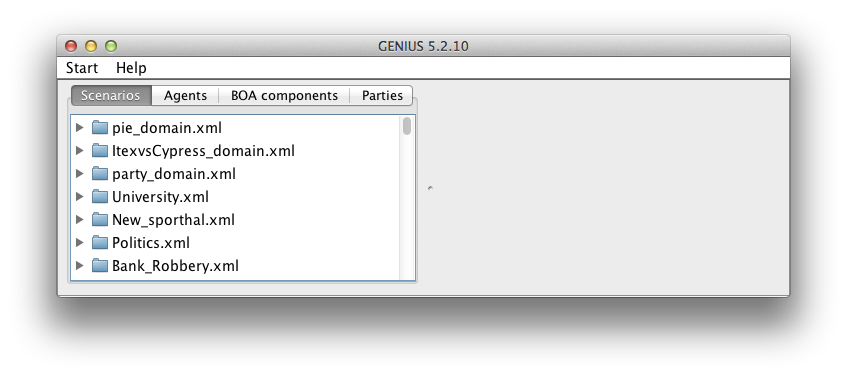
\includegraphics[width=0.6\textwidth]{media/start.png}
\caption{\Genius right after start-up. The left half is the components panel, the right half the status panel.}\label{Fig:negosimulator start}
\end{figure}


Progress messages and error messages are printed mainly to the standard output. On Mac OSX you can view these messages by opening the console window (double-click on Systemdisk/Applications/Utilities/Console.app). On Windows this is not directly possible. Console output can be read only if you start the application from the console window by hand, as follows. Go to the directory with the genius-XXX.jar and enter
\texttt{java -jar genius-XXX.jar}.
This will start the simulator, and all messages will appear in the console window. You may see some errors and warnings that are non-critical.

In some rare cases, agents and scenarios require more memory than allocated by default to Java. This problem can be resolved by using the Xmx and Xms parameters when launching the executable jar, for example \texttt{java -Xmx1536M -Xms1536M -jar genius-XXX.jar}. But usually, if your agent runs out of memory then there is some design flaw or bug. Competitions usually are run with the default amount of java memory so it is recommended to ensure that your  agent performs properly without requiring additional memory.

Please refer to chapter \ref{sec:debugging} for instructions on running \Genius in debug mode to debug your agent.

%=========================================================================================
\section{Scenario Creation}
A negotiation can be modeled in \Genius by creating a scenario. A scenario consists of a domain specifying the possible bids and a set of preference profiles corresponding to the preferences of the bids in the domain. This section discusses how to create a domain and a preference profile.


\subsection{Creating a Domain}
By right clicking on the list of available scenarios in the Components Window a popup menu with the option to create a new domain is shown. After clicking this option it is requested how the domain should be called. Next the domain is automatically created and a window similar to Figure~\ref{Fig:newdomain} is shown. Initially, a domain contains zero issues. We can simply add an issue by pressing the ``Add issue'' button. This results in the opening of a dialog similar to Figure~\ref{fig:createIssueD}.

\begin{figure}[htb]
	\centering
	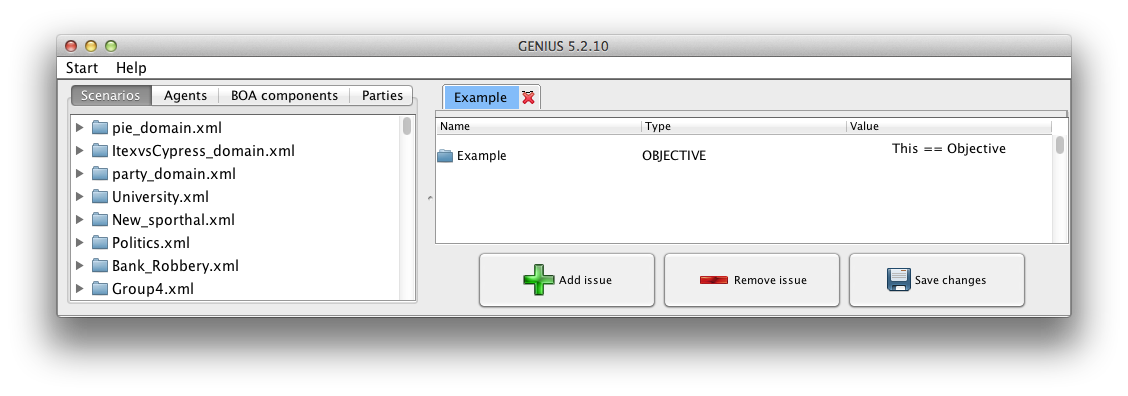
\includegraphics[width=0.9\textwidth]{media/exampledomain.png}
\caption{\Genius after creating a new Example domain.}\label{Fig:newdomain}
\end{figure}

The current version of \Genius~supports the creation of discrete and integer issues. Starting with a discrete issue, the values of the issue should be specified. In Figure~\ref{fig:createIssueD} we show the values of the issue ``Harddisk''. Note the empty evaluation values window, later on when creating a preference profile we will use this tab to specify the preference of each value.

Instead of a discrete issue, we can also add an integer issue as shown in Figure~\ref{fig:createIssueI}. For an integer issue we first need to specify the lowest possible value and the highest value, for example the price range for a second hand car may be $[500, 700]$. Next, when creating a preference profile we need to specify the utility of the lowest possible value (500) and the highest value (700). During the negotiation we can offer any value for the issue within the specified range.

The next step is to press ``Ok'' to add the issue. Generally, a domain consists of multiple issues. We can simply add the other issues by repeating the process above. If you are satisfied with the domain, you can save it by pressing  ``Save changes''.

Finally, note that the issues of a domain can only be edited if the scenario does not (yet) specify preference profiles. This is to avoid inconsistencies between the preference profiles and the domains. 

\begin{figure}[ht]
\center
\begin{minipage}[b]{0.35\linewidth}
	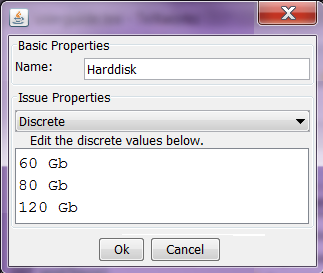
\includegraphics[width=0.95\textwidth]{media/image7a.png}
\caption{Creating a discrete issue.}
\label{fig:createIssueD}
\end{minipage}
\begin{minipage}[b]{0.55\linewidth}
	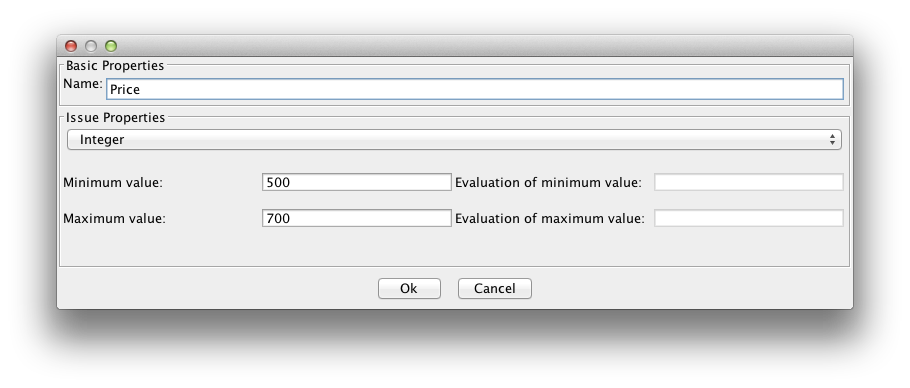
\includegraphics[width=1.0\textwidth]{media/image7b.png}
\caption{Creating an integer issue.}\label{fig:createIssueI}
\end{minipage}
\end{figure}

\subsection{Creating a Preference Profile}
Now that we created a domain, the next step is to add a set of preference profiles. Make sure that your domain is correct before proceeding, as \textbf{the domain can not be changed when it contains profiles}. By right clicking on the domain a popup menu is opened which has an option to create a new preference profile. Selecting this option results in the opening of a new window which looks similar to Figure~\ref{fig:utilcreated}.

\begin{figure}[htb]
	\centering
	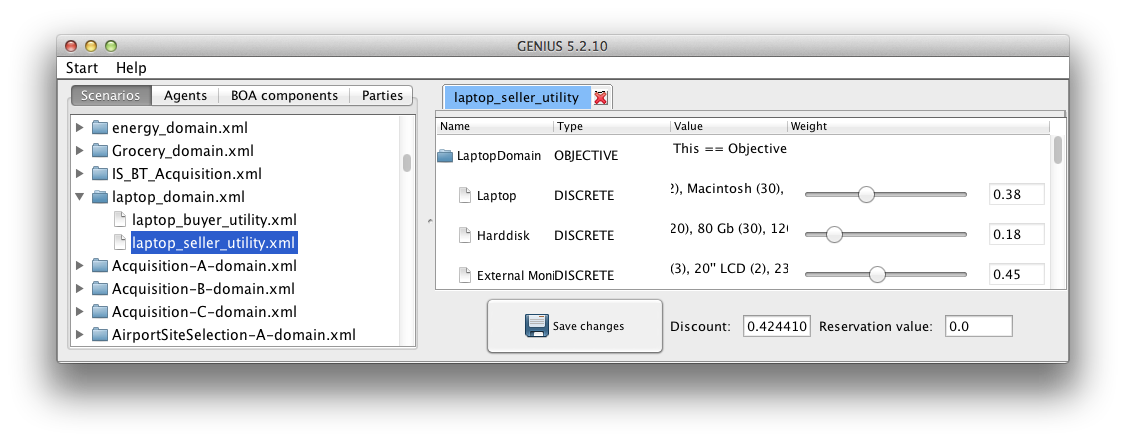
\includegraphics[width=0.8\textwidth]{media/laptop.png}
\caption{\Genius after creating a new utility space.}\label{fig:utilcreated}
\end{figure}

Now you are ready to start customizing the preference profile. There are three steps: setting the importance of the issues, determining the preference of the values of the issues, and configuring the reservation value and discount. To start with the first step, you can adjust the relative weights of the issues by using the sliders next to that issue. Note that when you move a slider, the weights of the other sliders are automatically updated such that the all weights still sum up to one. If you do not want that the weight of another issue automatically changes, you can lock its weight by selecting the checkbox behind it. Now that we set the weights of the issues, it is a good idea to save the utility space.

The next and final step is to set the evaluation of the issues. To specify the evaluation of an issue you can double click it to open a new window looking similar to Figure~\ref{fig:createIssueD} or Figure~\ref{fig:createIssueI} depending on the type of the issue.

For a discrete issue we need to specify the evaluation value of each discrete value. A specific value can be assigned any positive non-zero integer as evaluation value. During the negotiation the utility of a value is determined by dividing the value by the highest value for that particular issue. To illustrate, if we give 60 Gb evaluation 5, 80 Gb evaluation 8, and 120 Gb evaluation 10; then the utilities of these values are respectively 0.5, 0.8, and 1.0.

Specifying the preference of a integer issue is even easier. In this case we simply need to specify the utility of the lowest possible value and the highest possible value. The utility of a value in this range is calculated during the negotiation by using linear interpolation of the utilities of both given utilities.

The final step is to set the reservation value and discount of a preference profile. If you are satisfied with the profile you can save it by pressing ``Save changes''. Finally, you can create additional preference profiles for the domain and run a negotiation.


%=========================================================================================
\section{Running Negotiations}
This section discusses how to run a negotiation. There are two modes to run a negotiation:

\begin{itemize}
	\item \textbf{Multi-Party Negotiation}. A single negotiation session in which a number of agents (not necessarily 2) compete.
	\item \textbf{Multi-Party Tournament}. A tournament of multiparty sessions.
	
\end{itemize}

Before going into detail on how each of these modes work, we first discuss the two types of agents that can be used: automated agents and non-automated agents. Automated agents are agents that can compete against other agents in a negotiation without relying on input by a user. In general, these agents are able to make a large amount of bids in a limited amount of time.

In contrast, non-automated agents are agents that are fully controlled by the user. These types of agents ask the user each round which action they should make. \Genius~by default includes the UIAgent -- which has a simple user interface -- and the more extensive Extended UIAgent.


\subsection{Running a Multi-Party Negotiation Session}\label{sec:singlesessionrun}
To run a negotiation session select the menu ``Start'' and then ``Multi-Party Negotiation''. This opens a window similar to Figure~\ref{Fig:multipartysession}. 

\begin{figure}[h!]
	\centering
	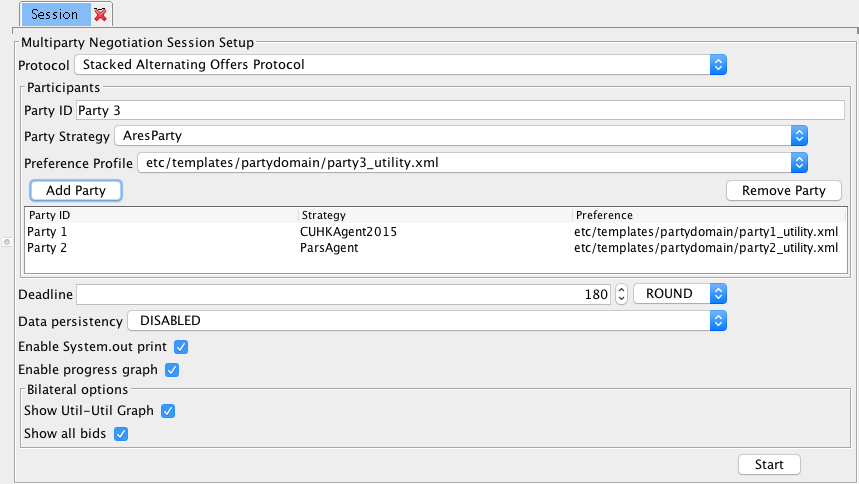
\includegraphics[width=0.5\textwidth]{media/multipartysession.png}
\caption{A multi-party negotiation session.}\label{Fig:multipartysession}
\end{figure}

The following parameters need to be specified to run a negotiation:

\medskip
\begin{minipage}{.8 \textwidth}
\begin{itemize}
	\item \textbf{Negotiation protocol}. The set of available protocols. See Chapter \ref{sec:protocols}.
	\item \textbf{Mediator}. The mediator ID and strategy that is to be used for this session. This is only visible if the protocol uses a mediator.
	\item \textbf{Participant Information}. The information (ID, strategy, profile) for the a party in the session. This information is copied into the table of participants when you click "Add Party".
	\item \textbf{A table with participants}. This table shows all currently added participants. You can add a party by setting the participant information above, and then clicking "Add Party". You can remove a party by selecting the party to remove in the table, and then clicking "Remove Party". 
	\item \textbf{Deadline}. The deadline to use. Can be "Round" or "Time". This determines the maximum duration of the session.
	\item \textbf{Data Persistency}. What kind of persistent data is available to the parties. The options are discussed in section \ref{sec:sessiongeneration}.
	\item \textbf{Enable System.out print}. If disabled, all system.out.print is suppressed during the negotiation. This is useful if for instance agents are flooding the output console, slowing down the system.
		\item \textbf{Enable progress graph}. If enabled (default), a progress chart is shown during the negotiation. You can disable this e.g. if the drawing is slowing down the system.
\item \textbf{Bilateral options} These appear only if you have exactly 2 parties added. The sub-options of this panel are
	\begin{itemize}
	\item \textbf{Show Util-Util Graph}. If enabled, the progress panel will show a graph where the utilities of the 2 parties are set along the X and Y axes. Also, the pareto frontier and nash point are shown in this graph. If disabled, it will show the default: a graph where the utilities of all parties are along the Y axis, and the time along the X axis. 
	\item \textbf{Show all bids}.  If enabled, and if 'Show Util-Util Graph' is enabled, this will show all the possible bids in the Util-Util graph.
	\end{itemize}

\end{itemize}
\end{minipage}
\medskip


The negotiation is started when you press the start button. The tab contents will change to  a progress overview panel
showing you the results of the negotiation (Figure \ref{fig:biprogress} and Figure \ref{fig:multiprogress}). The results are also stored in a log file.
 These results can be easily analyzed by importing them into Excel (cf. Section~\ref{sec:analysisExcel})

	\begin{figure}[ht]
		\center
		\begin{minipage}[b]{0.4\linewidth}
			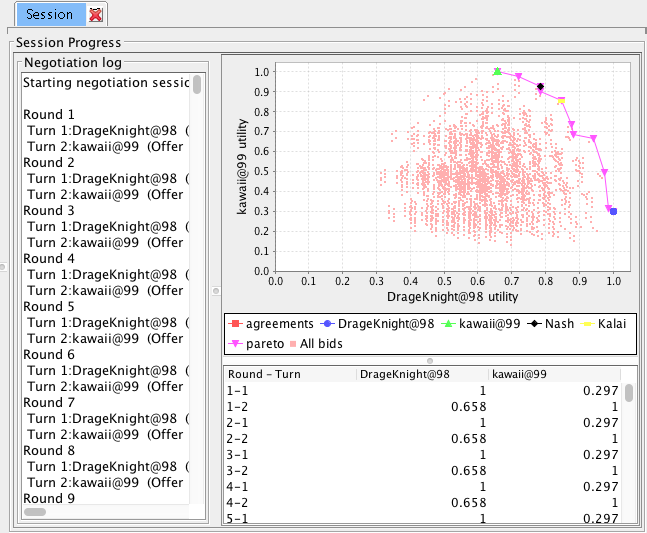
\includegraphics[width=0.95\textwidth]{media/bilateralprogress.png}
		\caption{Bilateral progress panel.}
		\label{fig:biprogress}
		\end{minipage}
		\begin{minipage}[b]{0.4\linewidth}
			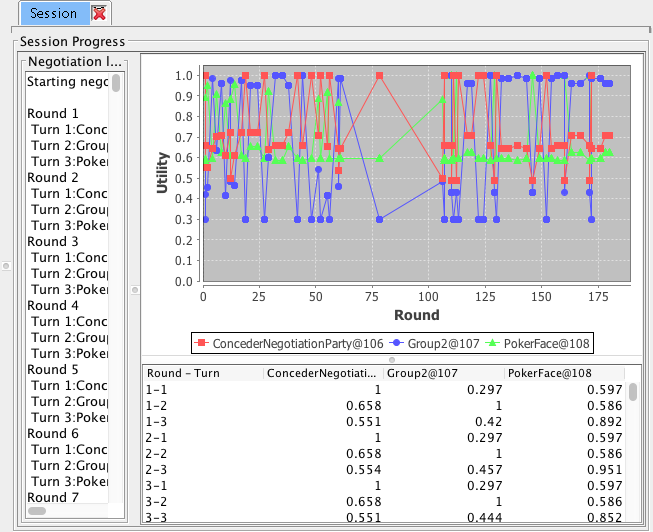
\includegraphics[width=0.95\textwidth]{media/multilateralprogress.png}
		\caption{Multilateral progress.}\label{fig:multiprogress}
		\end{minipage}
		\end{figure}
		

\subsection{Running a Multi-Party Tournament}
A multi-party tournament is a set of multi-party sessions. To prepare a multi-party tournament, select  ``Start'' and then ``Multi-Party Tournament''. 

\begin{figure}[htb]
	\centering
	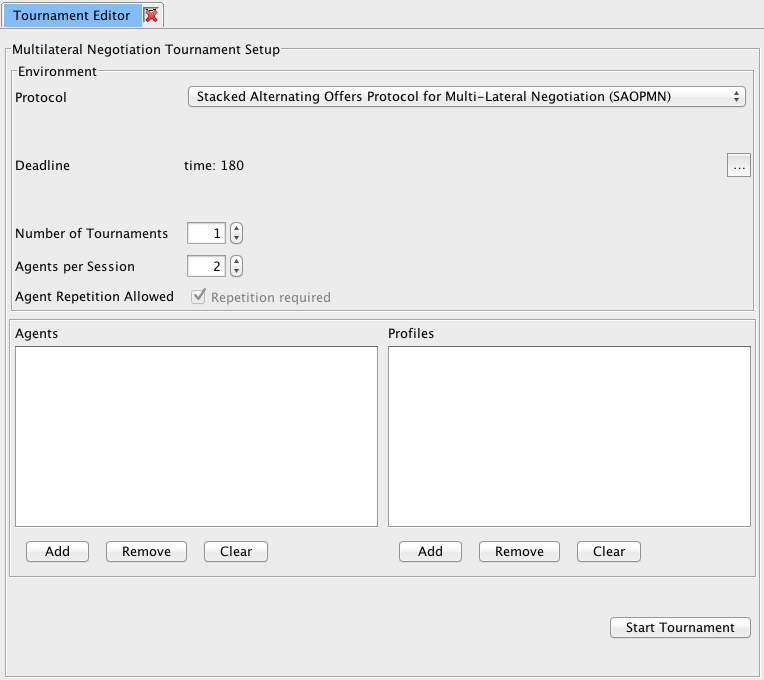
\includegraphics[width=0.7\textwidth]{media/multipartytournament.png}
\caption{Multi-Party Tournament}\label{Fig:multipartytournament}
\end{figure}

The Tournament tab will appear similar to Figure~\ref{Fig:multipartytournament}. This panel shows a set of tournament options. The detailed meaning of all these settings is explained in \ref{sec:sessiongeneration}.

\begin{itemize}
	\item \textbf{Protocol}. The protocol to use for each session.
	\item \textbf{Deadline}. The limits on time and number of rounds for each session.
	\item \textbf{Number of tournaments}. The number of times the entire tournament will be run.
	\item \textbf{Agents per Session}. The number of agents N to use for each session.
	\item \textbf{Agent Repetition}. whether to draw parties with or without return.
	\item \textbf{Randomize session order}. whether to randomize the session order
	\item \textbf{Data persistency}. The type of persistent data available to the parties. Same options as in section \ref{sec:singlesessionrun}.
	\item \textbf{Mediator}. The mediator to use. This option is visible only if the selected protocol needs a mediator. 
	\item \textbf{Agents}. The pool of agents to draw from. Click or drag in the agents area to (de)select agents. Click "Clear" to clear the pool.
	\item \textbf{Profiles}. The profiles pool. Click or drag in the profiles area to (de)select agents. Click "Clear" to clear the pool.
	\item \textbf{Special bilateral options}. These options appear only if Agents per session is set to 2 and is discussed in below .
\end{itemize}



\subsubsection{Bilateral special options}
If you have set 'Agents per session' to 2, and deselect 'Agent play both sides', you get an additional panel where you can select different Agents and Profiles for the B side of the 2-sided negotiation as in Figure~\ref{Fig:multipartytournament2}. 

\begin{figure}[htb]
	\centering
	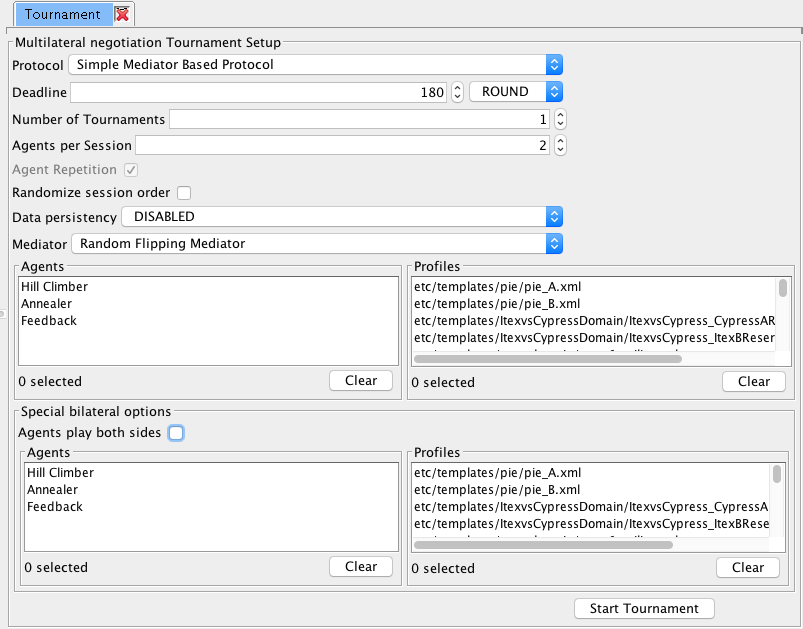
\includegraphics[width=0.7\textwidth]{media/multipartytournament2.png}
\caption{Multi-Party Bilateral Tournament}\label{Fig:multipartytournament2}
\end{figure}

After you click "Start Tournament", the tournament starts. The panel then is swapped for a tournament progress panel (Figure \ref{Fig:tournamentprogress}). 
In the top there is a progress bar showing the total number of sessions and the current session. The table shows all session results. The table is also saved to a $.csv$ log file in the log directory.

\begin{figure}[htb]
	\centering
	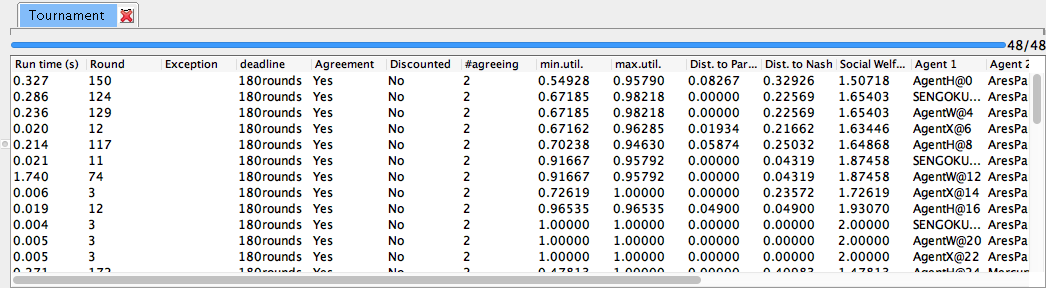
\includegraphics[width=0.9\textwidth]{media/tournamentprogress.png}
\caption{Tournament Progress panel}\label{Fig:tournamentprogress}
\end{figure}

The results of the tournament are shown on screen and also stored in a log file.  These results can be easily analyzed by importing them into Excel (cf. Section~\ref{sec:analysisExcel})


\subsection{Running from the command line}
You can run a multi-party tournament from the command line, as follows.

\begin{enumerate}
\item Prepare an xml file that describes the settings for the tournament
\item Run the command runner and give it the prepared file 
\end{enumerate}

\subsubsection{Prepare the XML settings file}
The first step is to create an xml file containing the values needed for session generation (Section \ref{sec:sessiongeneration}).
Make a copy of the \verb|multilateraltournament.xml| file inside your genius directory and edit it (with a plain text editor).  Inside the \verb|<tournaments>| element you will find a number of \verb|<tournament>| elements. Each of these \verb|<tournament>| elements defines a complete tournament so you can run multiple tournaments using one xml file.

The contents of each \verb|<tournament>| element is as follows. The meaning of the fields is detailed in section \ref{sec:sessiongeneration}.

\begin{itemize}
\item \textbf{protocolItem}. Contains the protocol to use, in the form of a protocolItem.
\item \textbf{deadline}.  the Deadline value.
\item \textbf{repeats}. the repeats value. 
\item \textbf{persistentDataType}. The type of the persistent data.
\item \textbf{numberOfPartiesPerSession}. the Parties per session value.
\item  \textbf{repetitionAllowed}. the value for the Party Repetition. 
\item \textbf{partyRepItems}. This element contains a number of \verb|<item>| elements. Each of these party items contains a description of a party as discussed below.
\item \textbf{mediator}. the mediator, if needed. This is similar in contents to a party item discussed below. 
 \item \textbf{partyProfileItems}. This element contains a number of items. There must be at least as much as numberOfNonMediatorsPerSession. 
 \end{itemize}

We have a number of items:
\begin{itemize}

\item A profile item : contains 
	 \begin{itemize}
	\item \textbf{url} that contains the description of that party profile. These URIs point to files and therefore are of the form \verb|file:path/to/file.xml|
  	\end{itemize}

\item A party item  (and mediator) contains:
  \begin{itemize}
    \item \textbf{classPath} the java.party.class.path to the main class. That class must implement the NegotiationParty interface
    \item \textbf{properties} can contain a number of \verb|<property>| nodes with these values
    		\begin{itemize}
		\item isMediator: this property indicates the party item is a mediator. If not set, the party will be 
		run as a normal party instead of a mediator, which will probably cause protocol violations
		\end{itemize}
  \end{itemize}

\item protocol item. This item contains the protocol information: 
	\begin{itemize}
	\item \textbf{hasMediator} which is true iff protocol requires mediator
	\item \textbf{description} a one-line textual description of the mediator
	\item \textbf{classPath} the java full.class.path of the protocol class
	\item \textbf{protocolName} a brief protocol name 
	\end{itemize}
\end{itemize}



The tournament will consist of sessions created creating all permutations of \verb|<numberOfNonMediatorsPerSession>| from the partyRepItems (with or without reuse, depending on \textbf{repetitionAllowed}. The randomization also is applied to the profile items.


\subsubsection{Run the tournament}
To run the tournament, open a terminal/console and change the working directory to the genius directory.
Then enter this command (where yourfile.xml is the name of the file you just edited and XXX the version of genius that you use):

\vspace{0.5cm}
\verb|java -cp genius-XXX-jar-with-dependencies.jar genius.cli.Runner yourfile.xml|
\vspace{0.5cm}

Press return if the app prompts you for the log file location to log to  the default \verb|logs/...csv| file.

\subsection{Tournament Session Generation}\label{sec:sessiongeneration}
Instead of manually setting all the setting, a tournament generates the exact session settings from the tournament settings. These
settings are specified either in the user interface settings, or in an XML file. The parameters are:

\begin{itemize}
\item \textbf{Protocol} The protocol value is used for all sessions. See section \ref{sec:protocols}.
\item \textbf{Mediator} The mediator to use for all sessions (ignored if the protocol does not need a mediator)
\item \textbf{Deadline} The deadline is used for all sessions.  A deadline contains two values:
     \begin{itemize}
        \item \textbf{value}. This is the maximum value determining the deadline. Must be an integer $\ge 1$.
        \item \textbf{type.} Can be either $ROUND$ or $TIME$. If $ROUND$, the value is the number of rounds. If $TIME$, value is a time in seconds.
      \end{itemize}
\item \textbf{Data persistency}. The type of persistent data available to the parties. The next time an agent of the same class and same profile runs in a tournament, it will receive the previously stored data. The options are 
	\begin{itemize}
	\item \textbf{Disabled}. Parties do not receive any persistent data. This is the default.
	\item \textbf{Serializable}. Parties can save anything serializable in the $PersistentDataContainer$.
	\item \textbf{Standard}. Parties receive a prepared, read only StandardInfo object inside the $PersistentDataContainer$.. 
	\end{itemize}
\item \textbf{repeats} This is also called 'number of tournaments' and determines the number of times a complete tournament will be run.
\item \textbf{Randomize Session Order} Whether all generated sessions within a tournament must be randomized.
\item \textbf{Parties per session} The number of agents to draw for each session. This excludes a possible mediator.
\item \textbf{Party Repetition} true if agents are to be drawn from the agents pool with return, false if they are to be drawn without return.
\item \textbf{Parties and Profile pool for side A}  A list from which parties and profiles will be drawn
\item \textbf{Parties and Profile pool for side B} Another list of parties and profiles. Only used with bilateral generation (see below).
\end{itemize}

The tournament generation works as follows. 

If there are exactly 2 agents per session and the agents and profiles for side B have been set, then bilateral generation is used. Otherwise, multilateral generation is used. This generation method creates an ordered list of sessions for 1 tournament.  If the 'Randomize Session Order' is set, the list is randomized. All sessions use the same protocol, mediator, deadline and data persistency.
This generation is called repeatedly, as set in 'repeats', and all generated session lists are accumulated in a big session list. This is the final result of the  tournament generation.

\subsubsection{Multilateral generation}
In multilateral generation,  all possible combinations of parties and profiles (using pool A) are generated as follows. the indicated number of parties per session $N$ are drawn from agent pool A, with our without return as specified in 'Party Repetition'. Also, $N$ profile items are drawn, ordered without return, from the profiles pool. These two lists are then paired into groups of $N$ party-profile pairs. 

\subsubsection{Bilateral generation}
In bilateral generation, first a set of participants P of all combinations of 1 party and 1 profile are drawn from the side A pool. Similarly a set of participants Q is drawn for the B pool. Then, the sessions set consists of all combinations of one participant from P and another participant from Q . 





%=========================================================================================
\section{Quality Measures in Genius}\label{sec:qm}
A large set of quality measures have been incorporated in \Genius~ since version 4.0. Most quality measures are automatically available, while for others an option must be selected in the tournament options menu.

There are  three types of logs used in \Genius: the standard log, the tournament log and the tournament statistics log.
\begin{itemize}
\item The standard log captures the outcome of each negotiation in a tournament by logging the results of the quality measures for both agents.
\item The tournament log uses the standard log to calculate averages and standard deviations of functions of the quality measures in the standard log, for example the average final utility for all sessions which resulted in an agreement.
\item The Tournament statistics log is logged only for the Multiparty Tournament. The file is written in the \verb|logs/| directory when the tournament finishes. It has the same filename as the tournament log, but with an additions "Stats". It contains statistics for each agent in the tournament.
\end{itemize}

First, Section~\ref{sec:standardLog} discusses the measures incorporated in the standard log. Next, Section~\ref{sec:tournamentLog} details the tournament log. Finally, Section~\ref{sec:analysisExcel} discusses how Excel can be used to analyze logs.

\subsection{Overview of Quality Measures in the Standard Log}\label{sec:standardLog}
Since version 4.0, \Genius~ incorporates two types of quality measures: standard measures and detailed measures. In addition there are some experimental measure types, such as competitiveness and opponent model accuracy, however these are not discussed here. In the following sections we discuss both measure types in detail.

\subsubsection{Standard Measures}
The standard measures are the measures which are enabled by default and cannot be disabled. Table~\ref{tab:standardmeasures} provides an overview of all default quality measures.

\begin{table}[h!]
	\small
	\center
	\begin{tabular}{|p{4.7cm}|p{9.2cm}|}
		\hline\hline
		\textbf{Attribute} & \textbf{Description}\\[-0.2ex] 
		\hline\hline
		acceptance\_strategy & The acceptance strategy of a BOA agent~(see Section~\ref{sec:boa}). \\[-0.2ex]\hline
		agent & The side at which the agent played (A or B). \\[-0.2ex]\hline
		agentClass & The classpath of the agent. \\[-0.2ex]\hline
		agentName & The name of the agent. \\[-0.2ex]\hline
		bestAcceptableBid & Utility of the best bid offered to the agent. Note that the discount is not taken into account. \\[-0.2ex]\hline
		bestDiscountedAccepableBid & Utility of the best bid offered to the agent, taking the discount into account. \\[-0.2ex]\hline
		bids & Amount of offers exchanged during the negotiation. \\[-0.2ex]\hline
		currentTime & Time of storage of the result of the negotiation. \\[-0.2ex]\hline
		discountedUtility & The discounted utility earned by the agent in the negotiation. \\[-0.3ex]\hline
		domain & Domain at which the negotiation took place.\\[-0.3ex]\hline
		errors & Errors encountered during the negotiation. Not reaching an agreement before the deadline is also treated as an error.\\[-0.3ex]\hline
		finalUtility & The undiscounted utility earned by the agent in the negotiation.\\[-0.3ex]\hline
		lastAction & Last action made before the negotiation ended.\\[-0.3ex]\hline
		normalized\_utility & The final utility divided by the maximum possible utility according to the preference profile. In correct domains the result should be equal to the final utility.\\[-0.3ex]\hline
		offering\_strategy & The offering strategy of a BOA agent~(see Section~\ref{sec:boa}). \\[-0.3ex]\hline
		opponent-agentClass & The classpath of the opponent.\\[-0.3ex]\hline
		opponent-agentName & The name of opponent's agent.\\[-0.3ex]\hline
		opponent\_model & The opponent model of a BOA agent~(see Section~\ref{sec:boa}). \\[-0.3ex]\hline
		opponent-utilSpace & The opponent's preference profile.\\[-0.3ex]\hline
		runNumber & How many times the negotiation has been repeated before.\\[-0.3ex]\hline
		startingAgent & Side which started the negotiation: A or B.\\[-0.3ex]\hline
		timeOfAgreement & Normalized time at which an agreement was established. 1.0 for no agreement. \\[-0.3ex]\hline
		utilSpace & The agent's preference profile.\\[-0.3ex]
		\hline
		\hline
	\end{tabular}
	\caption{Standard quality measures in \Genius in alphabetic order.}
	\label{tab:standardmeasures}
\end{table}

\subsubsection{Detailed Measures}\label{sec:detailedmeasures}
The detailed quality measures consist of trajectory analysis measures and measures for the fairness and optimality of the outcome. The detailed measures can be enabled by selecting ``Log detailed analysis'' in the tournament options menu. Enabling this option also results in the generation of the tournament log discussed in Section~\ref{sec:tournamentLog}.

\begin{table}[h!]
	\small
	\center
	\begin{tabular}{|p{4.7cm}|p{9.2cm}|}
		\hline\hline
		\textbf{Attribute} & \textbf{Description}\\[-0.2ex] 
		\hline\hline
		concession\_moves & The percentage of moves in which the agent, relative to the previous offer, offered a bid with decreased its own utility and increased its opponent's utility.\\[-0.3ex]\hline
		exploration\_rate & The percentage of bids in the outcome space explored by the agent. Two bids with exactly the same utilities for both parties are treated as a single same bid.\\[-0.3ex]\hline
		fortunate\_moves & The percentage of moves in which the agent, relative to the previous offer, offered a bid which increased both its own and its opponent's utility.\\[-0.3ex]\hline
		joint\_exploration\_bids & The percentage of unique bids of the outcome space explored by both agents together. Two bids with exactly the same utilities for both parties are treated as a single same bid. \\[-0.3ex]\hline
		kalai\_distance & Distance from the undiscounted utilities of the outcome to the Kalai-Smorodinsky solution.\\[-0.3ex]\hline
		nash\_distance & Distance from the undiscounted utilities of the outcome to the Nash solution. \\[-0.3ex]\hline
		nice\_moves & The percentage of moves in which the agent, relative to the previous offer, offered a bid which increased its opponent's utility without significantly changing its own utility.\\[-0.3ex]\hline
		pareto\_distance & Distance from the undiscounted utilities of the outcome to the nearest bid on the Pareto-optimal frontier.\\[-0.3ex]\hline
		perc\_pareto\_bids & Percentage of Pareto-optimal bids offered by an agent.\\[-0.3ex]\hline
		selfish\_moves & The percentage of moves in which the agent, relative to the previous offer, offered a bid which increased its own utility and decreased its opponent's utility.\\[-0.3ex]\hline
		silent\_moves & The percentage of moves in which the agent, relative to the previous offer, offered a bid which which was (nearly) equally valued by both agents.\\[-0.3ex]\hline
		social\_welfare & A fairness measure being the sum of the utilities for both agents.\\[-0.3ex]\hline
		unfortunate\_moves & The percentage of moves in which the agent, relative to the previous offer, offered a bid which decreased both its own and its opponent's utility.\\[-0.3ex]
		\hline
		\hline
	\end{tabular}
	\caption{Detailed quality measures in \Genius~in alphabetic order.}
	\label{tab:detailedMeasures}
\end{table}

\begin{comment}
\subsubsection{Opponent Model Accuracy Measures}
Log final accuracy

\begin{table}[h!]
\small
	\center
\begin{tabular}{|p{4.7cm}|p{9.2cm}|}
\hline
\textbf{Attribute} &\textbf{Description}\\
\hline\hline
\textsl{Pearson\_Correlation\_Bids} & Pearson correlation coefficient between real and estimated preference profile.\\
\hline
\textsl{Ranking\_Distance\_Bids} & Ranking distance between real and estimated preference profile.\\
\hline
\textsl{Average\_Difference\_Bids} & Average difference between the real and estimated utility of each possible bid.\\
\hline
\textsl{Ranking\_Distance\_Issue\_Weights} & Ranking distance between real and estimated issue weights.\\
\hline
\textsl{Average\_Difference\_Issue\_Weights} & Average difference between the real and estimated issue weights.\\
\hline
\textsl{Kalai\_Difference} & Difference between the real and estimated utility of the Kalai-point.\\
\hline
\textsl{Nash\_Diference} & Difference between the real and estimated utility of the Nash-point.\\
\hline
\textsl{Difference\_Pareto\_Frontier} & The average difference between the real and estimated utility for each Pareto bid.\\
\hline
\textsl{Percentage\_Correct\_Pareto\_Bids} & Percentage of real Pareto bids which are also estimated to be a Pareto bid.\\
\hline
\textsl{Percentage\_Incorrect\_Pareto\_Bids} & Percentage of estimated Pareto bids which are also real Pareto bids.\\
\hline
\textsl{Pareto\_Frontier\_Distance} & First, the position of the estimated Pareto bids is determined in the real space. The value of the measure is the absolute difference in surface under the real Pareto bids and the bids estimated to be Pareto optimal.\\ % absolute, because if a point is missed, then surface of estimate can actually be larger. Note that this case is rare
\hline
\end{tabular}
	\caption{Opponent model accuracy measures in \Genius~in alphabetic order.}
	\label{tab:omaccuracyMeasures}
\end{table} 
\end{comment}

\subsection{Overview of Quality Measures in the Tournament Log}~\label{sec:tournamentLog}
The tournament log is an analysis of the results on the quality measures for each agent, for example the average utility for \textit{Agent K}. Similar to the detailed quality measured the tournament log can be enabled by selecting ``Log detailed analysis'' in the tournament options menu.

Three types of measures are included in the log:
\begin{itemize}
	\item \textbf{Averages of quality measures}. The tournament log includes a large set of averages of the quality measures in the standard log. Examples include the average Nash distance, the average percentage of silent moves, and the average social welfare.
	\item \textbf{Standard deviations of quality measures}. The tournament log also includes the standard deviation of some measures. Note that this not the normal standard deviation of for example the utility, but the more complicated deviation between runs. To illustrate, if there were ten runs of the tournament, then each run has an average utility and we can calculate the standard deviation of this utility between runs.
	\item \textbf{Average of functions of quality measures}. The tournament log also includes a large set of measures which are functions of measures included in the standard log. An example is the average utility for an agent only for the matches which resulted in agreement. 
\end{itemize}

\subsection{Analyzing Logs using Excel}~\label{sec:analysisExcel}
The logs are in XML format, which entails that we can easily analyze them by using Excel. Note that the following discussion does not apply to the starter edition of Excel, as it does not support Pivot tables.

The XML data of the standard log can be converted to a normal table by importing the data into Excel using the default options. This results in a large table showing the result for both agents A and B for each session. Analyzing these results manually is complicated, therefore we recommend to use pivot tables. Pivot tables allow to summarize a large set of data using statistics and can be created by selecting ``Insert'' and then ``Pivot Table''. To illustrate, by dragging the \textit{agentName} in ``Row Labels'' and the \textit{discountedUtility} in ``Values'' (see Figure~\ref{fig:pivottable}), we can easily see which agent scored best in the tournament. If solely the amount of matches of each agent is displayed, you need to set the ``Value Field Settings'' of \textit{discountedUtility} to average instead of count.

\begin{figure}[htb]
	\centering
	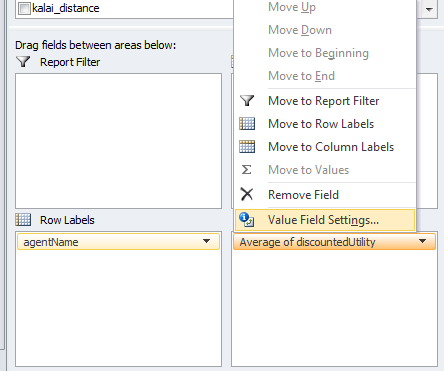
\includegraphics[width=0.4\textwidth]{media/PivotTable.png}
\caption{Configuration required to summarize the discounted utility of each agent.}\label{fig:pivottable}
\end{figure}


%=========================================================================================

\section{Creating a Negotiation Agent}\label{sec:createagent}
This section discusses how to create a negotiation agent in Java. These agents can negotiate with any number of parties. 

\subsection{Set up your workspace}
In order to compile your agent  you need to set up a workspace. 
We assume 
\begin{itemize}
\item Java 8 SDK and Eclipse has been installed
\item the developer has knowledge about Eclipse and Java, 
\item The developer has some basic knowledge of the maven-eclipse integration. 
\end{itemize}

The following steps are done in Eclipse:

\begin{enumerate}
\item Select in the workbench File/New Project... and select Maven/new Maven project. 
\item Select "create a simple project" and click next. Enter some group id (eg "ai2019") and some artifactID (eg "group20"). Click finish.
\item open the pom.xml file inside your new project and insert this inside the \verb|<project>| part:

\begin{verbatim}
   <dependencies>
      <dependency>
         <groupId>genius</groupId>
         <artifactId>core</artifactId>
         <version>1.0.1</version>
      </dependency>
   </dependencies>

   <repositories>
      <repository>
         <id>artifactory.ewi.tudelft.nl</id>
         <url>http://artifactory.ewi.tudelft.nl/artifactory/libs-release</url>
      </repository>
      <repository>
         <id>netbeans</id>
         <name>Netbeans rep</name>
         <url>http://bits.netbeans.org/maven2/</url>
      </repository>
   </repositories>
\end{verbatim}

\item Add/edit your agent under \verb|src/main/java|.  For a quick start, you can just copy the entire multypartyexample folder (available in the \Genius zip file you downloaded when installing) into src/main/java.
\end{enumerate}
 \FloatBarrier

Eclipse now automatically downloads and includes all dependencies into your project and build your agent into target/classes. 



\subsection{Example agents}
The \Genius zip file contains two examples: the Multiparty example and the Storage example

The multiparty example just accepts any acceptable bid with a random probability of 0.5. 

The storage example demonstrates using the persistent data storage. This example is showing how the storage can be used to wait a little longer every next time the party is in a negotiation.

To run this example, you need to set up \Genius to allow persistent data storage (the default is off). In the \Genius tournament setup panel, use the following settings
\begin{itemize}
\item  number of tournaments= 20
\item   agents per session =2
\item  persistency=standard
\item  agent side A: GroupX, \verb|party1_utility.xml|
\item  agent side B: Random Party, \verb|party6_utility.xml|
\end{itemize}

and start the tournament and check the number of rounds till agreement: it will increase every session.

Now run another tournament with the same settings but pick select both \verb|party1_utility.xml| and \verb|party2_utility.xml|. Run the tournament.
Now you will see that the the number of rounds till agreement goes up every other run. This is because your agent gets a different profile every other run and thus there are persistent data stores, one for each profile. 




\subsection{Implementing NegotiationParty}
This section discusses details of implementing a NegotiationParty.  

Every agent must at least implement the \texttt{negotiator.parties.NegotiationParty} interface (Table \ref{table:NegotiationPartyInterface}),  Also the implementation must have a public default (no-argument) constructor. Please refer to the javadocs for details on the parameters.

\begin{table*}[t]
  \centering
  \begin{tabular}{|p{4cm}|p{7cm}|}
  \hline
  Method & description \\
  \hline\hline
    init &Initializes the party, informing it of many negotiation details. This is be called exactly once by the negotiation system, immediately after construction of the class  \\
    chooseAction & When this function is called, it is expected that the Party chooses one  of the actions from the possible action list and returns an instance of the chosen action. \\
    receiveMessage & This method is called to inform the party that another NegotiationParty chose an Action.\\
    getDescription & Returns a human-readable description for this party \\
    getProtocol & The actual supported MultilateralProtocol. Usually this returns StackedAlternatingOffersProtocol.\\
    negotiationEnded & This is called to inform the agent that the negotiation has been ended. This allows the agent to record some final conclusions about the run\\
    \hline
  \end{tabular}
  \caption{Methods of NegotiationParty. Check the javadoc for all the details}
  \label{table:NegotiationPartyInterface}
\end{table*}

For convenience, you can also extend the class \texttt{negotiator.parties.AbstractNegotiationParty}. This class provides convenient support functions for building your agent. 

Your agent might need to check the provided AbstractUtilitySpace, for instance if your agent supports for example only AdditiveutilitySpace.

We recommend to use the javadoc included with the distribution to check the details of all the involved classes. 

\FloatBarrier


The examples extend AbstractNegotiationParty which is a basic implementation of NegotiationParty. Table \ref{tab:agentclass} shows the most important fields and methods of this class. For more information, please refer to the javadoc of \Genius.

\begin{table}[h]
\begin{tabular}{m{0.9\textwidth}}
\hline
\texttt{void init(NegotiationInfo info)}\\
Informs the agent about beginning of a new negotiation session.\\
\hline
\texttt{NegotiationInfo}\\
The context of the negotiation: the utility space, the timeline and deadline, the agentID and persistent data container.\\
\hline
\texttt{UtilitySpace}\\
The preference profile of the scenario allocated to the agent.\\
\hline
\texttt{Timeline }\\
Use timeline for every time-related by using \texttt{getTime()}.\\
\texttt{Action chooseAction(List<Class<? extends Action>> possibleActions)}\\
This function should return the action your agent wants to make next.\\
\hline
\texttt{Action}\\
Superclass of negotiation actions like Offer, Accept and EndNegotiation..\\
\hline
\texttt{void receiveMessage(AgentID sender, Action action)}\\
Informs the agent which action the opponent did.\\
\hline
\end{tabular}
\caption{The most important methods and fields of the NegotiationParty class.}
\label{tab:agentclass}
\end{table}

\subsubsection{Receiving the Opponent's Action}\label{sec:receiveAction}
The \texttt{ReceiveMessage(Action opponentAction)} informs you that the opponent just performed the action \texttt{opponentAction}. The \texttt{opponentAction} may be  \texttt{null} if you are the first to place a bid, or an \texttt{Offer}, \texttt{Accept} or \texttt{EndNegotiation} action.
The \texttt{chooseAction()} asks you to specify an \texttt{Action} to send to the opponent.

In the SimpleAgent code, the following code is available for \texttt{receiveMessage}. The SimpleAgent stores the opponent's action to use it when choosing an action.

\begin{lstlisting}
public void receiveMessage(Action opponentAction) {
	actionOfPartner = opponentAction;
}
\end{lstlisting}

\subsubsection{Choosing an Action}\label{sec:chooseAction}
The code block below shows the code of the method \texttt{chooseAction} for SimpleAgent. For safety, all code was wrapped in a try-catch block, because if our code would accidentally contain a bug we still want to return a good action (failure to do so is a protocol error and results in a utility of 0.0).

The sample code works as follows. If we are the first to place a bid, we place a random bid with sufficient utility (see the .java file for the details on that). Else, we determine the probability to accept the bid, depending on the utility of the offered bid and the remaining time. Finally, we randomly accept or pose a new random bid.

While this strategy works, in general it will lead to suboptimal results as it does not take the opponent into account. More advanced agents try to model the opponent's strategy or preference profile.

\begin{lstlisting}
public Action chooseAction() {
	Action action = null;
	Bid partnerBid = null;
	try {
		if (actionOfPartner == null)
			action = chooseRandomBidAction();
		if (actionOfPartner instanceof Offer) {
			partnerBid = ((Offer) actionOfPartner).getBid();
			double offeredUtilFromOpponent = getUtility(partnerBid);
			double time = timeline.getTime();
			action = chooseRandomBidAction();
			Bid myBid = ((Offer) action).getBid();
			double myOfferedUtil = getUtility(myBid);
			// accept under certain circumstances
			if (isAcceptable(offeredUtilFromOpponent, myOfferedUtil, time))
				action = new Accept(getAgentID(), partnerBid);
		}
		if (timeline.getType().equals(Timeline.Type.Time)) {
			sleep(0.005); // just for fun
		}
	} catch (Exception e) {
		 // best guess if things go wrong. Notice this may still fail
		action = new Accept(getAgentID(), partnerBid);
	}
	return action;
}
\end{lstlisting}

The method \textit{isAcceptable} implements the probabilistic acceptance function$P_\text{accept}$:

\begin{equation}
	P_\text{accept} = \dfrac{u - 2ut + 2\left(t - 1 + \sqrt{(t - 1)^2 + u(2t - 1)}\right)}{2t - 1}
\end{equation}
where $u$ is the utility of the bid made by the opponent (as measured in our utility space), and $t$ is the current time as a fraction of the total available time. Figure~\ref{Fig:Paccept} shows how this function behaves depending on the utility and remaining time. Note that this function only decides if a bid is acceptable or not. More advanced acceptance strategies also use the \texttt{EndNegotiation} action.
\begin{figure}[htb]
	\centering
	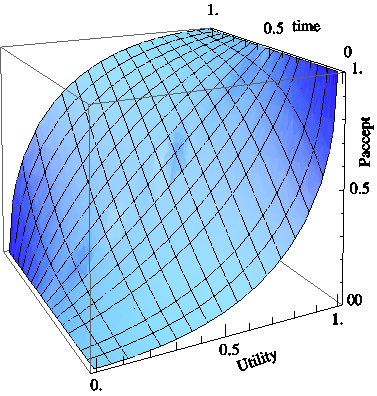
\includegraphics[width=0.3\textwidth]{media/image21.png}
	\caption{$P_\text{accept}$ value as function of the utility and time (as a fraction of the total available time).}\label{Fig:Paccept}
\end{figure}
 

\subsubsection{Overview of useful Classes}
This section provides an overview of classes which might be useful when implementing an agent. For the documentation of the data structures that are presented, please refer to the Javadoc that can be found in your download of \Genius. 

\begin{itemize}

\item \textbf{BidDetails} is a structure to store a bid and its utility.
\item \textbf{BidHistory} is a structure to keep track of the bids presented by the agent and the opponent.
\item \textbf{BidIterator} is a class used to enumerate all possible bids. Also refer to \textit{SortedOutcomeSpace}.
\item \textbf{BidSpace} is a class which can be used to determine the Pareto-optimal frontier and outcomes such as the Nash solution. This class can be used with the opponent's utility space as estimated by an opponent model.
\item \textbf{Pair} is a simple pair of two objects.
\item \textbf{Range} is a structure used to describe a continuous range.
\item \textbf{SortedOutcomeSpace} is a structure which stores all possible bids and their utilities by using BidIterator. In addition, it implements efficient search algorithms that can be used to search the space of possible bids for bids near a given utility or within a given utility range.
\item \textbf{UtilitySpace} is a representation of a preference profile. It is recommended to use this class when implementing a model of the opponent's preference profile.
\end{itemize}



\subsection{Loading a NegotiationParty}

You need to load your custom party into the \Genius party repository in order to use it. After adding, your agent will appear in the combo boxes in the multilateral tournament runner and session runner where you can select the party to use.

Locate the Parties repository tab in the GUI (Figure \ref{fig:partiesrepo}). Right click in this area and select "Add Party". A file browser panel pops up. Browse to  your compiled \verb|.class| file that implements the NegotiationParty and select it. Typically maven compiles into \verb|target/classes|. Your party will appear at the bottom of the parties repository. The \verb|partyrepository.xml| file is automatically updated accordingly.

\begin{figure}[h!] 
	\center
	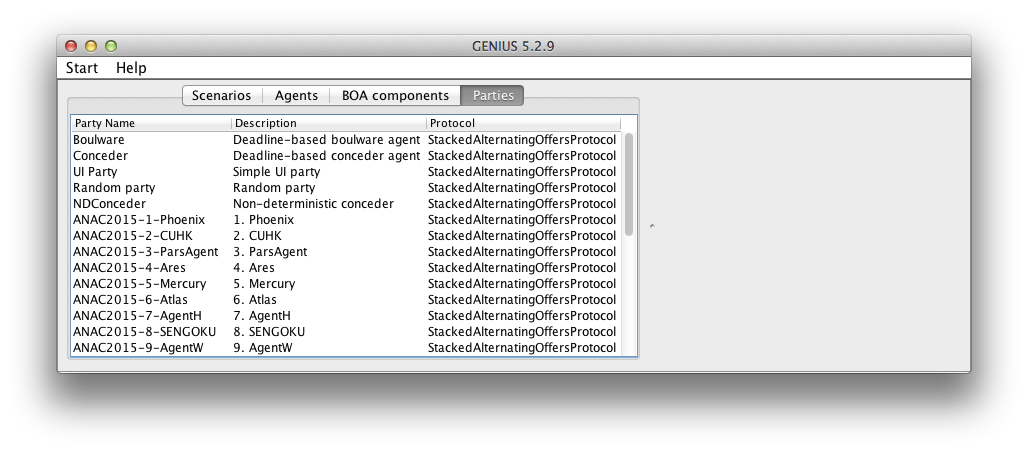
\includegraphics[width=10cm]{media/partiesrepo.png}
	\caption{The parties repository.}
	\label{fig:partiesrepo}
\end{figure}


To do this manually without using the GUI, quit \Genius, open the \verb|partyrepository.xml| file \footnote{This file is automatically created the first time you run \Genius}  and add a section like this

\begin{lstlisting}
<partyRepItem classPath="full.class.of.your.party" <properties/> />
\end{lstlisting}

After that you can restart \Genius so that it loads the new party.
\FloatBarrier

\subsection{Third party code}
You should not use maven to add dependencies, as Java 8 can not deal properly with multiple versions of the same library in within a JVM.

Instead, if you want to use a third party library, you will have to include all the source code of that library with your code, including all sub-dependencies. The code should be copied inside the package name of your agent, instead of using the original package name of that library (so do not use "org.apache" for instance). This is to ensure that we are really running your agent on the specific version of the library that your agent needs and to avoid version conflicts (java will run an unspecified version of the library in case of conficts). 


%=========================================================================================
\section{Creating a BOA Agent}\label{sec:boa}
Instead of implementing your negotiating agent from scratch, you can create a BOA agent using the \textit{BOA framework}.
The BOA negotiation agent architecture allows to reuse existing components from other BOA agents. Many of the sophisticated agent strategies that currently exist are comprised of a fixed set of modules. Generally, a distinction can be made between four different modules: one module that decides whether the opponent's bid is acceptable (\textit{acceptance strategy}); one that decides which set of bids could be proposed next (\textit{bidding strategy}); one that tries to guess the opponent's preferences (\textit{opponent model}), and finally a component which specifies how the opponent model is used to select a bid for the opponent (\textit{opponent model strategy}). The overall negotiation strategy is a result of the interaction between these components.

The advantages of separating the negotiation strategy into these four components (or equivalently, fitting an agent into the BOA framework) are threefold: first, it allows to \textit{study the performance of individual components}; second, it allows to \textit{systematically explore the space of possible negotiation strategies}; third, the reuse of existing components \textit{simplifies the creation of new negotiation strategies}.

BOA components can be used both in bilateral tournaments and multilateral negotiation (both single sessions and tournaments). 



\subsection{Components of the BOA Framework}
A negotiation agent in the BOA framework, called a \textit{BOA agent}, consists of four components:
\begin{description}
  \item[Bidding strategy] A bidding strategy is a mapping which maps a negotiation trace to a bid. The bidding strategy can interact with the opponent model by consulting with it.%, passing one or multiple bids and see how they compare within the opponent's utility space.

  \item[Opponent model] An opponent model is in the BOA framework a learning technique that constructs a model of the opponent's preference profile.% In our approach, the opponent model should be able to estimate the opponent's utility of a given bid.
  \item[Opponent model strategy] An opponent model strategy specifies how the opponent model is used to select a bid for the opponent and if the opponent model may be updated in a specific turn.
  \item[Acceptance strategy] The acceptance strategy determines whether the opponent's bid is acceptable and may even decide to prematurely end the negotiation.
\end{description}
The components interact in the following way (the full process is visualized in Figure~\ref{fig:flowchart}). When receiving a bid, the BOA agent first  updates the \textit{bidding history}. Next, the \textit{opponent model strategy} is consulted if the \textit{opponent model} may be updated this turn. If so, the \textit{opponent model} is updated.

Given the opponent's bid, the \textit{bidding strategy} determines the counter offer by first generating a set of bids with a similar preference for the agent. The \textit{bidding strategy} uses the \textit{opponent model strategy} to select a bid from this set taking the opponent's utility into account.

Finally, the \textit{acceptance strategy} decides whether the opponent's action should be accepted. If the opponent's bid is not accepted by the acceptance strategy, then the generated bid is offered instead.

\begin{figure}[t] 
	\center
	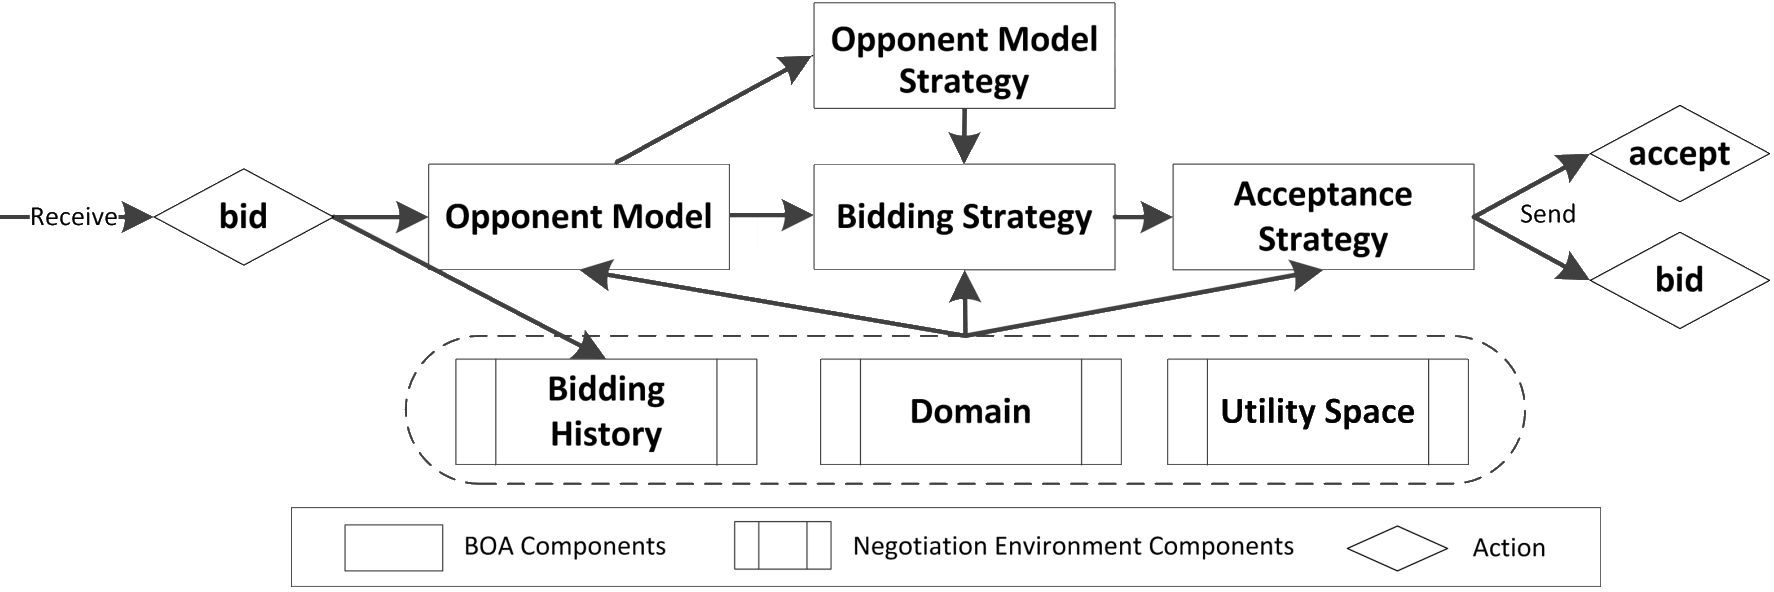
\includegraphics[width=15.0cm]{media/BOAflow.png}
	\caption{The BOA Framework Architecture.}
	\label{fig:flowchart}
\end{figure}


\subsection{Create a BOA Party}
For use in the mulit-ilateral negotiation system, the boa agents can be edited in the "Boa Parties" repository tab (Figure \ref{fig:boaparties}). Right-click in the panel to add items. Select an item and right-click to remove or edit an item.  These BOA parties are at this moment still a simple extension of the old bilateral system, and can \emph{only be used in multi-lateral negotiation with exactly 2 parties per session}.  


\begin{figure}[!ht] 
	\center
	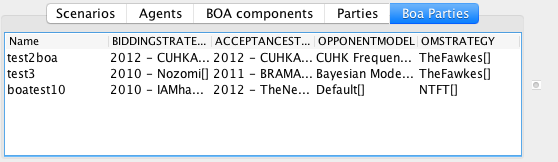
\includegraphics[width=10.0cm]{media/boacomponants.png}
	\caption{The BOA Parties repository tab.}
	\label{fig:boaparties}
\end{figure}


After you selected to add or edit a BOA party (Figure \ref{fig:editboaparty}).  Here you can select a different Bidding Strategy, Acceptance Strategy, Opponent Model and Opponent Model Strategy by selecting the appropriate strategy with the combo boxes. If the strategy has parameters, the current parameter settings are shown and the respective "Change" button enables.


\begin{figure}[!ht] 
	\center
	\includegraphics[width=10.0cm]{media/EditBoaParty.png}
	\caption{Editing a BOA party.}
	\label{fig:editboaparty}
\end{figure}

If you click on the  "Change" button, another panel pops up where you can edit the parameters (Figure \ref{fig:editparameters}). You can click directly in the table to edit values.

\begin{figure}[!ht] 
	\center
	\includegraphics[width=10.0cm]{media/EditParameters.png}
	\caption{Editing the Parameters of a BOA party.}
	\label{fig:editparameters}
\end{figure}

When you have correctly set all strategies and their parameters, you can click the "OK" button in the BOA party editor (Figure  \ref{fig:editboaparty}). Then, agents with the given name are generated, one for each permutation of the range of settings you set in the parameters. For example, if you set you want parameter m to have values 0,1 and 2 and x to have values 7 and 8, there will appear 6 new agents, with settings [0,7],[0,8],[1,7],[1,8],[2,7], and [2,8]. Be careful with this generation as it is easy to create an excessive amount of agents this way.

\subsection{Bi-Lateral BOA}

In this section we create a \textit{BOA agent} by selecting its components from a list of existing components. 

In the bilateral tournament runner you edit the BOA agents in the tournament settings, and the Boa Parties repository is ignored. The BOA framework GUI (see Figure~\ref{fig:decoupledGUI}) can be opened by double clicking the \textit{Values} section next to the \textit{BOA Agent side A} or \textit{BOA Agent side B} when creating a (distributed) tournament.




\begin{figure}[h!]
	\center
	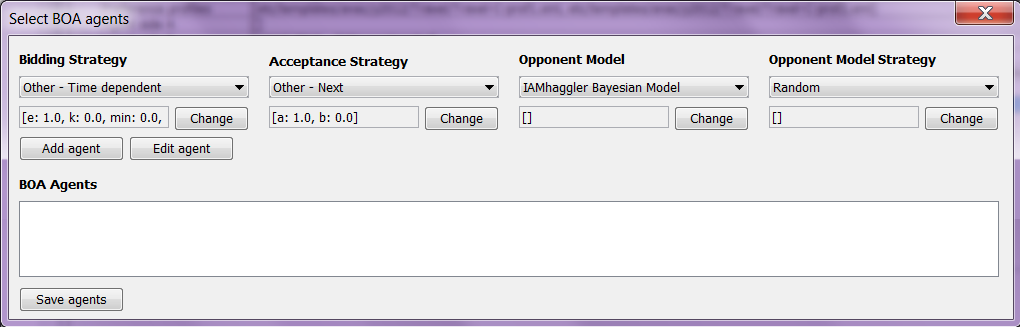
\includegraphics[width=15cm]{media/BOAgui.png}
	\caption{The BOA framework GUI.}
	\label{fig:decoupledGUI}
\end{figure}

Our goal in this section is to specify three BOA agents which are equal except for a single parameter $a$ of their acceptance strategy. 

To add the agents, click on the "Add agent(s)" button. A dialog pops up to enter the BOA agent details (Figure~\ref{fig:boadetails}).

\begin{figure}[h!]
	\center
	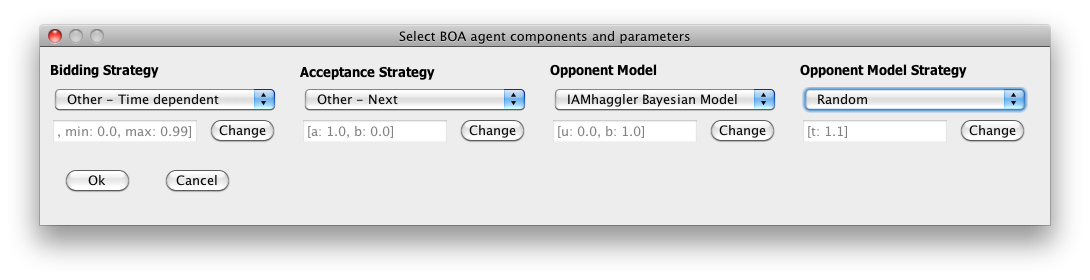
\includegraphics[width=15cm]{media/BOAdetails.png}
	\caption{The BOA agent components and parameters dialog.}
	\label{fig:boadetails}
\end{figure}

We select the bidding strategy \textit{Other - Time Dependent} under the heading \textit{Bidding Strategy}. Note that when we select this strategy, the default parameters of the component appear in the textbox below. Next, we select the other three components shown in Figure~\ref{fig:boadetails}.

The next step is to specify three variants of the acceptance strategy differing in the parameter $a$. To be more precise, we want $a$ to be 1.0, 1.1, and 1.2. To achieve this, press the ``Change'' button under  \textit{Acceptance Strategy}  to open a window similar to Figure~\ref{fig:boaparam}. Next, fill in the fields as shown in Figure~\ref{fig:boaparam}. Finally, we select ``Add agent(s)'' to create the three agents. Press "Save agents" to save the new BOA agents for the tournament. Note that in this example we only varied a single parameter of a single component. If we vary more parameters possibly of different components, then all possible combinations are generated.

\begin{figure}[h!] 
	\center
	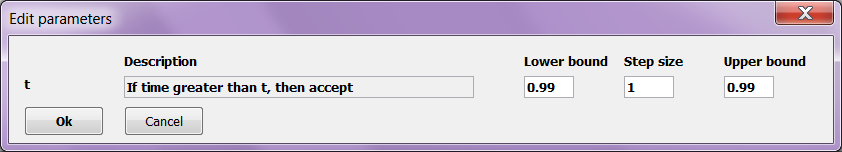
\includegraphics[width=15cm]{media/BOAparam.png}
	\caption{Adding a parameter.}
	\label{fig:boaparam}
\end{figure}

\subsection{Creating New Components}
This section discusses how create your own components. An example implementation of each component is included in the ``boaexamplepackage'' folder. The next section discusses how these components can be added to the list of available components in the BOA framework GUI.

\subsubsection{Parameters}
All BOA components have the same mechanism to be tuned with parameters. They should have no constructor : the default empty constructor will be called. They initialize through a call to init().

The parameters and their default parameters are indicated by the component by overriding the getParameters() function. This function should return a set of $BAOparameter$ objects, each parameter having a unique name, description and default value.


\begin{table}[h]
\begin{tabular}{m{0.9\textwidth}}
\hline
\texttt{public Set<BOAparameter> getParameterSpec() }\\
 Override this function to add parameters to the module.\\
\hline
\end{tabular}
\caption{The getParameters method. Override if your component has parameters.}
\label{tab:parameters}
\end{table}


When the component is actually used, the actual values for the parameters (which may differ from the default) are passed to the init function when the component is initialized.

\subsubsection{Creating a Bidding Strategy}
A bidding strategy can be easily created by extending the \textit{OfferingStrategy} class. Table~\ref{tab:BOAbs} depicts the methods which need to be overridden. The \textit{init} method of the bidding strategy is automatically called by the BOA framework with four parameters: the negotiation session, the opponent model, the opponent model strategy, and the parameters of the component. The negotiation session object keeps track of the negotiation state, which includes all offers made by both agents, the timeline, the preference profile, and the domain. The parameters object specifies the parameters as specified in the GUI. In the previous section we specified the parameter $b$ for the acceptance strategy $Other - Next$ to be 0.0. In this case the agent can retrieve the value of the parameter by calling \textit{parameters.get(``b'')}.

An approach often taken by many bidding strategies is to first generate all possible bids. This can be efficiently done by using the \textit{SortedOutcomeSpace} class. For an example on using this class see the \textit{TimeDependent\_Offering} class in the \textit{boaexamplepackage} directory.

\begin{table}[h]
\begin{tabular}{m{0.9\textwidth}}
\hline
\texttt{void init(NegotiationSession negotiationSession, OpponentModel opponentModel, 
	OMStrategy omStrategy, Map<String, Double> parameters)}\\
Method directly called after creating the agent which should be used to initialize the component.\\
\hline
\texttt{BidDetails determineOpeningBid()}\\
Method which determines the first bid to be offered to the component.\\
\hline
\texttt{BidDetails determineNextBid()}\\
Method which determines the bids offered to the opponent after the first bid.\\
\hline
\end{tabular}
\caption{The main methods of the bidding strategy component.}
\label{tab:BOAbs}
\end{table}


\subsubsection{Creating an Acceptance Condition}
This section discusses how to create an acceptance strategy class by extending the abstract class \textit{AcceptanceStrategy}. Table~\ref{tab:BOAas} depicts the two methods which need to specified.

\begin{table}[h]
\begin{tabular}{m{0.9\textwidth}}
\hline
\texttt{void init(NegotiationSession negotiationSession, OfferingStrategy offeringStrategy,
			OpponentModel opponentModel, Map<String, Double> parameters)}\\
Method directly called after creating the agent which should be used to initialize the component.\\
\hline
\texttt{Actions determineAcceptability()}\\
Method which determines if the agent should accept the opponent's bid (\textit{Actions.Accept}), reject it and send a counter offer (\textit{Actions.Reject}), or leave the negotiation (\textit{Actions.Break}).\\
\hline
\end{tabular}
\caption{The main methods of the acceptance strategy component.}
\label{tab:BOAas}
\end{table}

\subsubsection{Creating an Opponent Model}
This section discusses how to create an opponent model by extending the abstract class \textit{OpponentModel}. Table~\ref{tab:BOAom} provides an overview of the main methods which need to specified. For performance reasons it is recommended to use the \textit{UtilitySpace} class.

\begin{table}[h]
\begin{tabular}{m{0.9\textwidth}}
\hline
\texttt{void init(NegotiationSession negotiationSession, Map<String, Double> parameters)}\\
Method directly called after creating the agent which should be used to initialize the component.\\
\hline
\texttt{double getBidEvaluation(Bid bid)}\\
Returns the estimated utility of the given bid.\\
\hline
\texttt{double updateModel(Bid bid)}\\
Updates the opponent model using the given bid.\\
\hline
\texttt{UtilitySpace getOpponentUtilitySpace()}\\
Returns the opponent's preference profile. Use the \textit{UtilitySpaceAdapter} class when not using the UtilitySpace class for the opponent's preference profile.\\
\hline
\end{tabular}
\caption{The main methods of the opponent model component.}
\label{tab:BOAom}
\end{table}

\subsubsection{Creating an Opponent Model Strategy}
This section discusses how to create an opponent model strategy by extending the abstract class \textit{OMStrategy}. Table~\ref{tab:BOAoms} provides an overview of the main methods which need to specified.

\begin{table}[h]
\begin{tabular}{m{0.9\textwidth}}
\hline
\texttt{void init(NegotiationSession negotiationSession, OpponentModel model, Map<String, Double> parameters)}\\
Method directly called after creating the agent which should be used to initialize the component.\\
\hline
\texttt{BidDetails getBid(List<BidDetails> bidsInRange);}\\
This method returns a bid to be offered from a set of given similarly preferred bids by using the opponent model.\\
\hline
\texttt{boolean canUpdateOM();}\\
Determines if the opponent model may be updated this turn.\\
\hline
\end{tabular}
\caption{The main methods of the opponent model strategy component.}
\label{tab:BOAoms}
\end{table}

\subsection{Compiling BOA Components}
BOA components must be compiled before they can be loaded into Genius.
To compile a BOA component, do the following steps (in this example we compile the boa example components)
\begin{itemize}
\item Open a terminal 
\item Switch to the root directory of genius
\item \raggedright Enter the command \verb|javac -cp genius-XXX.jar -source 1.8 -target 1.8 boaexamplepackage/*.java |
\end{itemize}

You can also compile from Eclipse or Netbeans. Make sure you add the genius-XXX.jar to your class path. Please refer to the Eclipse or Netbeans documentation on how to do this.


\subsection{Adding a Component to the BOA Repository}
In the previous section we discussed how to create each type of BOA component. To use the components, we still need to add them to the \textit{BOA repository}. To do so, open the BOA components tab in the components window as shown in Figure~\ref{fig:boacomponents}. Right click and select ``Add new component''. This results in the opening of the window shown in Figure~\ref{fig:loadBOA}.

\begin{figure}[h!] 
	\center
	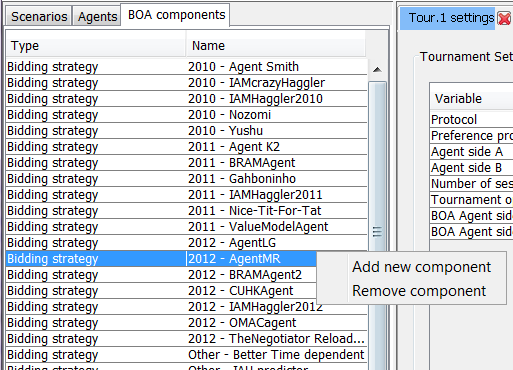
\includegraphics[width=7cm]{media/AddBOA.png}
	\caption{The BOA components window.}
	\label{fig:boacomponents}
\end{figure}

Click on the "Open" button and select the main class file of your BOA component (the class file that implements the BOA interface). Then check the name of the component, you can change it but it has to be a unique name in the registry. Optionally add parameters. Finally, clicking ``Add component'' in this window adds the component to the repository.

\begin{figure}[h!] 
	\center
	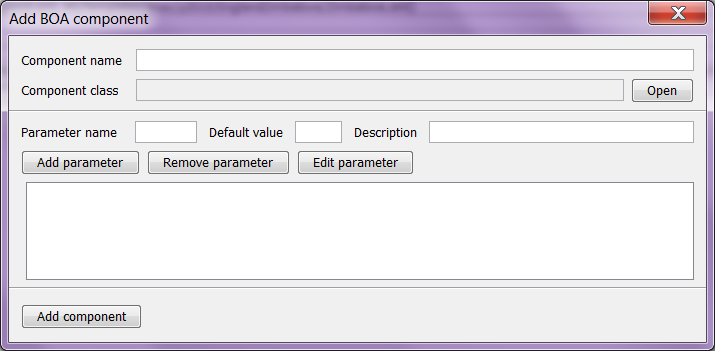
\includegraphics[width=5cm]{media/LoadBOA.png}
	\caption{Loading a BOA agent.}
	\label{fig:loadBOA}
\end{figure}


\subsection{Creating a ANAC2013 BOA Agent}\label{sec:anac2013agentBOA}
In Section~\ref{sec:anac2013agent} we discussed how to create an agent for the ANAC2013. Using a similar procedure it is also possible to create BOA agents compatible with ANAC2013. An example to do so is included in this distribution of \Genius.

As only a single object can be saved and loaded, the BOA framework stores an object \textit{SessionData} that includes the data saved by all three components. This object is loaded and saved automatically by the BOA framework. A component can easily access the data it saved by using the \textit{loadData} method. A component can at each moment during the negotiation update the saved information by using the \textit{storeData} method, although we recommend updating the information at the end of the negotiation by using the the \textit{endSession} method. The \textit{endSession} method of each method is automatically called at the end of the negotiation to inform the component of the result obtained and should be used to update the \textit{SessionData} object before it is automatically stored.

\subsection{Advanced: Converting a BOA Agent to an Agent}
To convert a BOA agent to a normal agent you have to create a class that extends \textit{BOA agent} and override the \textit{agentSetup} method. Below is an example of a BOA agent wrapped as a normal agent.

\begin{lstlisting}
public class SimpleBOAagent extends BOAagent{

	@Override
	public void agentSetup() {
		OpponentModel om = new FrequencyModel(negotiationSession, 0.2, 1);
		OMStrategy oms = new NullStrategy(negotiationSession);
		OfferingStrategy offering  = new TimeDependent_Offering(
			negotiationSession, om, oms, 0.2, 0, 1, 0);
		AcceptanceStrategy ac = 
			new AC_Next(negotiationSession, offering, 1, 0);
		setDecoupledComponents(ac, offering, om, oms);		
	}

	@Override
	public String getName() {
		return "SimpleBOAagent";
	}
}
\end{lstlisting}

\subsection{Advanced: Multi-Acceptance Criteria (MAC)}
The \textit{BOA framework} allows us to better explore a large space of negotiation strategies. MAC can be used to scale down the negotiation space, and thereby make it better computationally explorable.

As discussed in the introduction of this chapter, the acceptance condition determines solely if a bid should be accepted. This entails that it does not influence the bidding trace, except for when it is stopped. In fact, the only difference between \textit{BOA agents} where only the acceptance condition vary, is the time of agreement (assuming that the computational cost of the acceptance conditions are negligible).

Given this property, multiple acceptance criteria can be tested in parallel during the same negotiation trace. In practice, more than 50 variants of a simple acceptance condition as for example $\textbf{AC}_{next}$ can be tested in the same negotiation at a negligible computational cost.

To create a multi-acceptance condition component you first need to extend the class \textit{Mulit Acceptance Condition}, this gives access to the ACList which is a list of acceptance conditions to be tested in parallel. Furthermore, the method \textit{isMac} should be overwritten to return \textit{true} and the name of the components in the repository should be \textit{Multi Acceptance Criteria}. An acceptance can be added to the MAC by appending it to the AClist as shown below. 

\begin{lstlisting}[language=Java, caption={Example code for Acceptance condition}]
public class AC_MAC extends Multi_AcceptanceCondition {
	@Override
	public void init(NegotiationSession negoSession, 
			OfferingStrategy strat, OpponentModel opponentModel, 
			HashMap<String, Double> parameters) throws Exception {
		this.negotiationSession = negoSession;
		this.offeringStrategy = strat;
		outcomes = new ArrayList<OutcomeTuple> ();
		ACList = new ArrayList<AcceptanceStrategy>();
		for (int e = 0; e < 5; e++) {
			ACList.add(new AC_Next(negotiationSession, 
				offeringStrategy, 1, e * 0.01));
		}
	}
}
\end{lstlisting}




%=========================================================================================

\section{Debugging}\label{sec:debugging}
This section explains how to debug your agent using Eclipse. It is assumed you set up your agent already as in Chapter \ref{sec:createagent}.

To easily debug this agent from Genius, take the following steps:

\begin{enumerate}
\item Add this dependency to the pom
\begin{verbatim}
      <dependency>
         <groupId>genius</groupId>
         <artifactId>gui</artifactId>
         <version>8.0.0</version>
      </dependency>
\end{verbatim}
\item Right click on your project root and select \verb|Debug As/Java Application|
\item select \verb|Application - genius|.
\item Click "Ok".
\end{enumerate}

{\em NOTICE}: Your agent must compile also without this added dependency. This extra dependency is only to facilitate debugging in \Genius 

Once you have Genius running in Eclipse, you can simply place a breakpoint in your agent and run Genius from Eclipse in debug mode.

\subsection{Source code and javadocs}
Eclipse downloads all source codes and javadocs automatically. But if you like you can download these as a jar from \url{http://artifactory.ewi.tudelft.nl/artifactory/libs-release/genius/core/}. You can extract the files in the jar using \verb|jar -xf <file>.jar| or using your favorite unzip program.

\FloatBarrier



%%%%%%%%%%%%%%%%%%%%%%%%%%%%%%%%%%%%%%%%%%%%%%%%%%%%%%%%%%%%%%%%%%%%%%%%%%%%%%%%%%%



\section{Conclusion}
This concludes the manual of \Genius. If you experience problems or have suggestions on how to improve \Genius, please send them to \url{negotiation@ii.tudelft.nl}. 

\Genius\ is actively used in academic research. If you want to cite \Genius\ in your paper, please refer to \cite{Genius}.



\bibliographystyle{plain}
\bibliography{genius}

\end{document}